\section{Resultados}
\subsection{Servidor unak.is}

\begin{center}
\captionof{table}{rtt promedio entre saltos para unak.is}
\begin{tabular}{llllr}
\toprule
        &    &               &    &       rtt \\
host & ttl & ip & cc &           \\
\midrule
unak.is & 1  & empty & empty &  0.000000 \\
        & 2  & empty & empty &  0.000000 \\
        & 3  & empty & empty &  0.000000 \\
        & 4  & empty & empty &  0.000000 \\
        & 5  & 200.89.161.137 & AR &  0.074301 \\
        & 6  & 200.89.165.5 &  AR &  0.003707 \\
        & 7  & 200.89.165.250 & AR &  0.004276 \\
        & 8  & 190.216.88.33 & AR &  0.000000 \\
        &    & empty & empty &  0.000000 \\
        & 9  & 67.16.159.37 & US &  0.145690 \\
        & 10 & 64.57.20.73 & US &  0.005504 \\
        & 11 & 64.57.20.34 & US &  0.005281 \\
        & 12 & 64.57.20.37 & US &  0.010810 \\
        & 13 & empty & empty &  0.000000 \\
        & 14 & 109.105.97.142 & SE &  0.080042 \\
        & 15 & 109.105.97.138 & SE &  0.011689 \\
        & 16 & 109.105.97.125 & SE &  0.004030 \\
        & 17 & 109.105.102.1 & SE &  0.049820 \\
        & 18 & 130.208.17.162 & IS &  0.009160 \\
        & 19 & 130.208.17.58 & IS &  0.001856 \\
        & 20 & 130.208.18.106 & IS &  0.019887 \\
        & 21 & 130.208.224.102 & IS &  0.003169 \\
\bottomrule
\end{tabular}
\end{center}

\begin{center}
\begin{tabular}{p{6.5cm}r}
Porcentaje de saltos que no responden los $Time$ $exceeded$: & \textbf{28\%} \\ \\ 
Largo de la ruta en términos de saltos que responden: &\textbf{15 saltos} \\ \\
Cantidad de enlaces intercontinentales: & \textbf{1} \\ \\
Cantidad de outliers según el método de Cimbala: & \textbf{1} \\ \\
\end{tabular}
\end{center}

Los outliers se corresponden con los enlaces intercontinentales.


\begin{figure}[H]
  \centering
    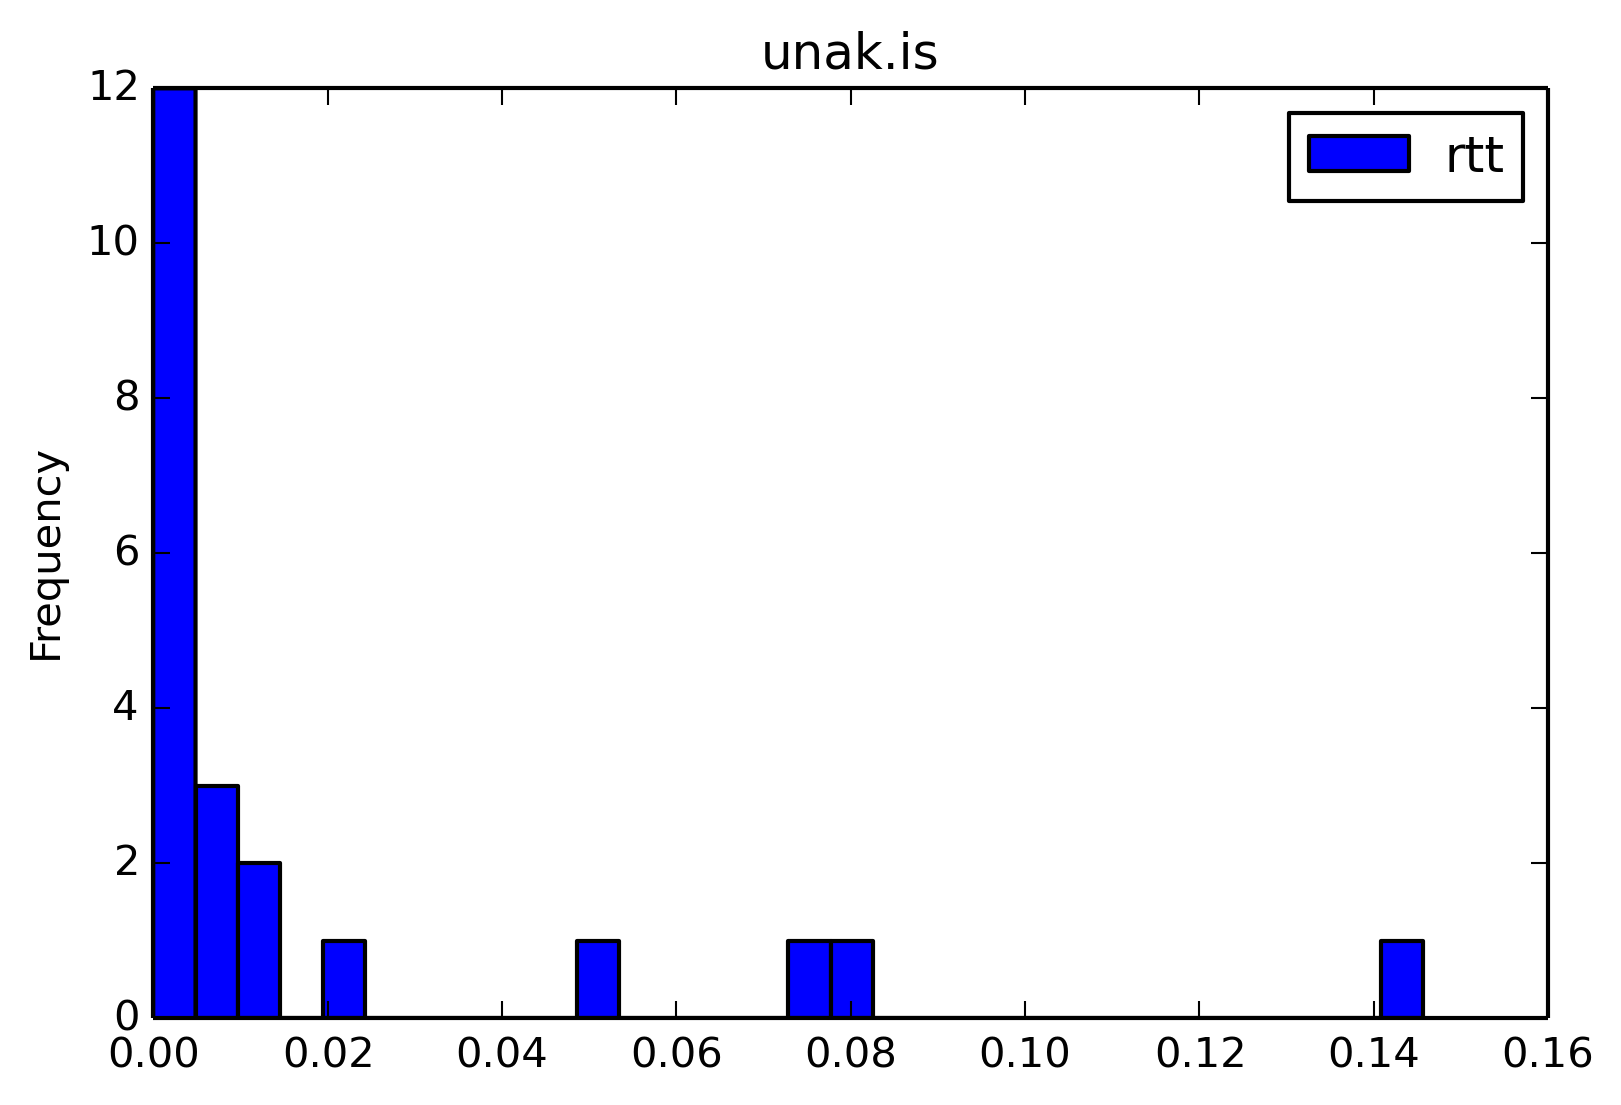
\includegraphics[width=0.45\textwidth]{histogramas_rtt/unak-is.png}
  \caption{RTT entre saltos}
  \label{entropia-s}
\end{figure}

\begin{center}
\captionof{table}{Outliers para unak.is}
\begin{tabular}{llllr}
\toprule
        &    &               &    &      rtt \\
host & ttl & ip & cc &          \\
\midrule
unak.is & 9  & 67.16.159.37 & US &  3.44859 \\
\bottomrule
\end{tabular}
\end{center}

\begin{figure}[H]
  \centering
    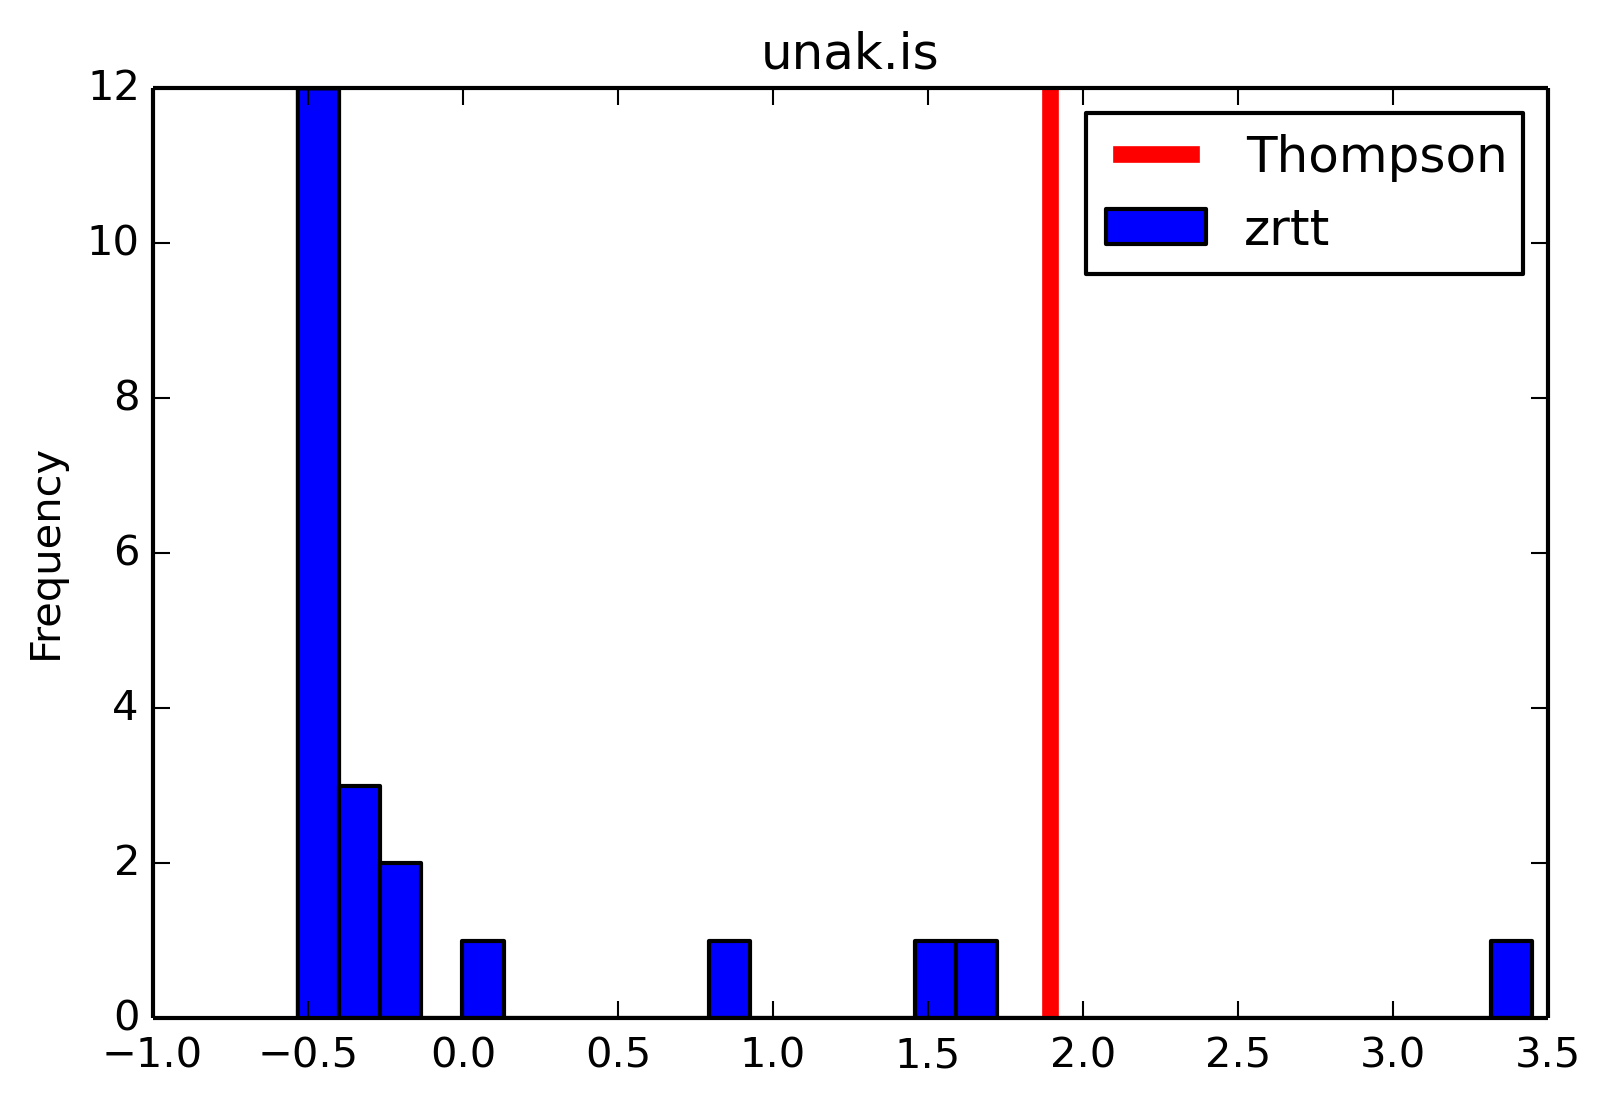
\includegraphics[width=0.45\textwidth]{histogramas_thompson/unak-is.png}
  \caption{RTT }
  \label{entropia-s}
\end{figure}

\begin{figure}[H]
  \centering
    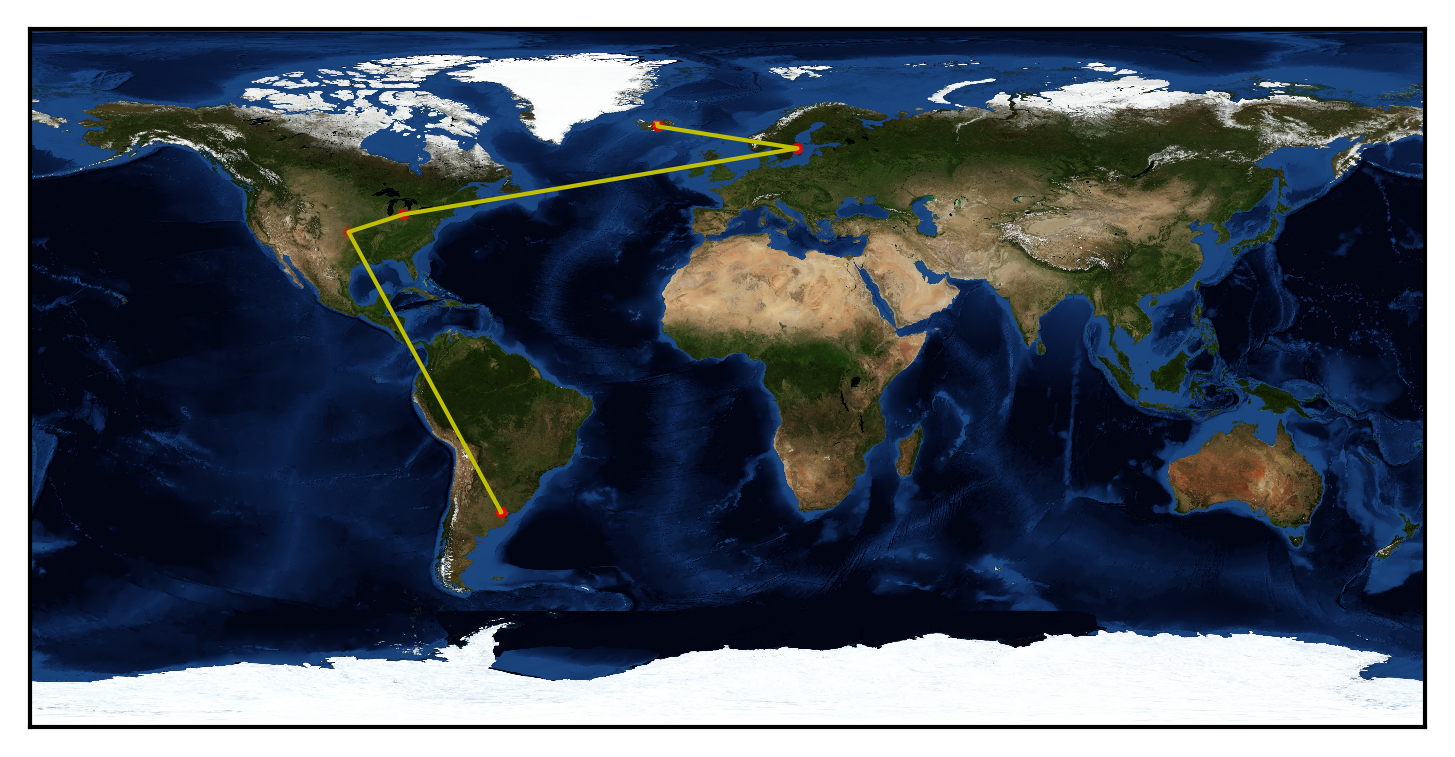
\includegraphics[width=0.45\textwidth]{grafico-rutas/unak-is.png}
  \caption{Gráfico de la ruta}
  \label{entropia-s}
\end{figure}



\subsection{Servidor unis.no}
\begin{center}
\captionof{table}{rtt promedios entre saltos para unis.no}
\begin{tabular}{llllr}
\toprule
        &    &                &    &       rtt \\
host & ttl & ip & cc &           \\
\midrule
unis.no & 1  & empty & empty &  0.000000 \\
        & 2  & empty & empty &  0.000000 \\
        & 3  & empty & empty &  0.000000 \\
        & 4  & empty & empty &  0.000000 \\
        & 5  & 200.89.161.97 & AR &  0.072603 \\
        & 6  & 200.89.165.1 & AR &  0.005187 \\
        & 7  & 200.89.165.250 & AR &  0.003868 \\
        & 8  & empty & empty &  0.000000 \\
        & 9  & 64.215.102.181 & US &  0.137360 \\
        & 10 & 64.57.20.73 & US &  0.008581 \\
        & 11 & 64.57.20.34 & US &  0.006402 \\
        & 12 & 64.57.20.37 & US &  0.008664 \\
        & 13 & empty & empty &  0.000000 \\
        & 14 & 109.105.97.142 & SE &  0.085971 \\
        & 15 & 109.105.97.138 & SE &  0.010124 \\
        & 16 & 109.105.102.66 & SE &  0.019075 \\
        & 17 & 109.105.102.67 & SE &  0.012499 \\
        & 18 & 128.39.255.121 & NO &  0.004408 \\
        & 19 & 128.39.255.47 & NO &  0.019374 \\
        & 20 & 128.39.255.211 & NO &  0.009346 \\
        & 21 & 128.39.255.19 & NO &  0.006287 \\
        & 22 & 128.39.254.85 & NO &  0.008778 \\
        & 23 & 128.39.47.158 & NO &  0.008459 \\
        & 24 & 158.39.149.250 & NO &  0.005062 \\
\bottomrule
\end{tabular}
\end{center}

\begin{center}
\begin{tabular}{p{6.5cm}r}
Porcentaje de saltos que no responden los $Time$ $exceeded$: & \textbf{25\%} \\ \\ 
Largo de la ruta en términos de saltos que responden: &\textbf{18 saltos} \\ \\
Cantidad de enlaces intercontinentales: & \textbf{1} \\ \\
Cantidad de outliers según el método de Cimbala: & \textbf{2} \\ \\
\end{tabular}
\end{center}

No se corresponden los enlaces con los outliers.

\begin{figure}[H]
  \centering
    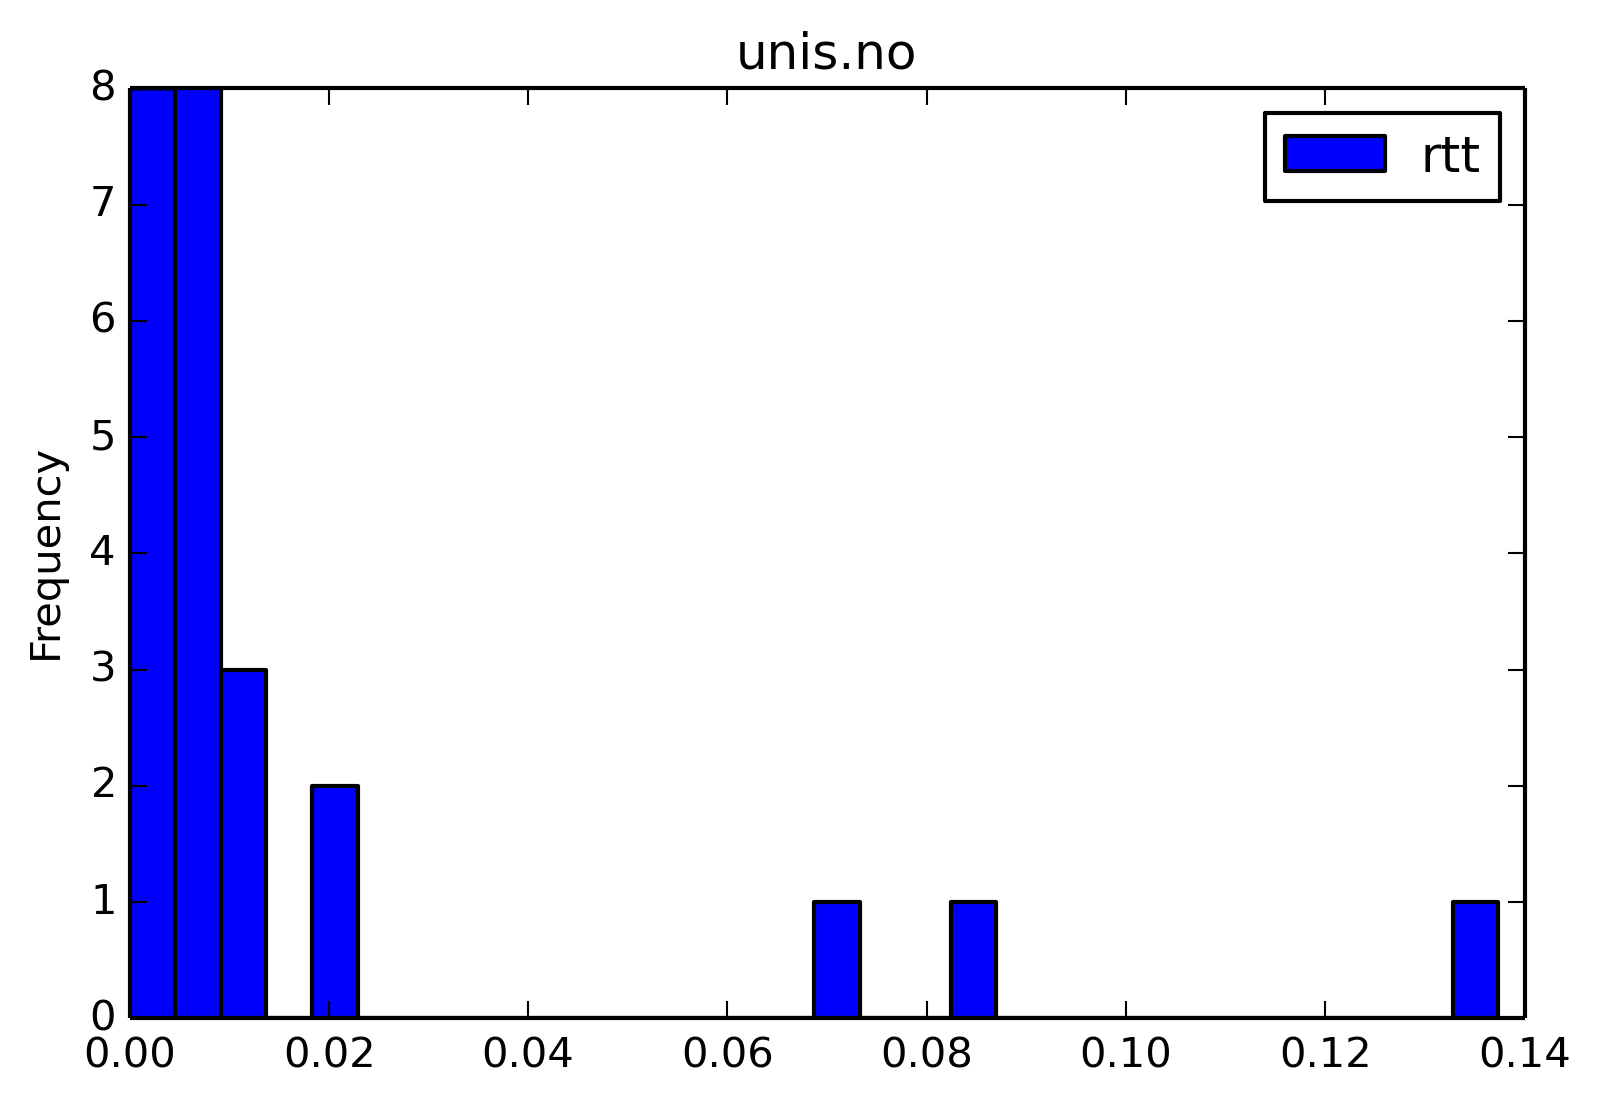
\includegraphics[width=0.45\textwidth]{histogramas_rtt/unis-no.png}
  \caption{RTT entre saltos}
  \label{entropia-s}
\end{figure}

\begin{center}\captionof{table}{Outliers para unis.no}

\begin{tabular}{llllr}
\toprule
        &    &                &    &       rtt \\
host & ttl & ip & cc &           \\
\midrule
unis.no & 9  & 64.215.102.181 & US &  3.598609 \\
        & 14 & 109.105.97.142 & SE &  2.049258 \\
\bottomrule
\end{tabular}

\end{center}

\begin{figure}[H]
  \centering
    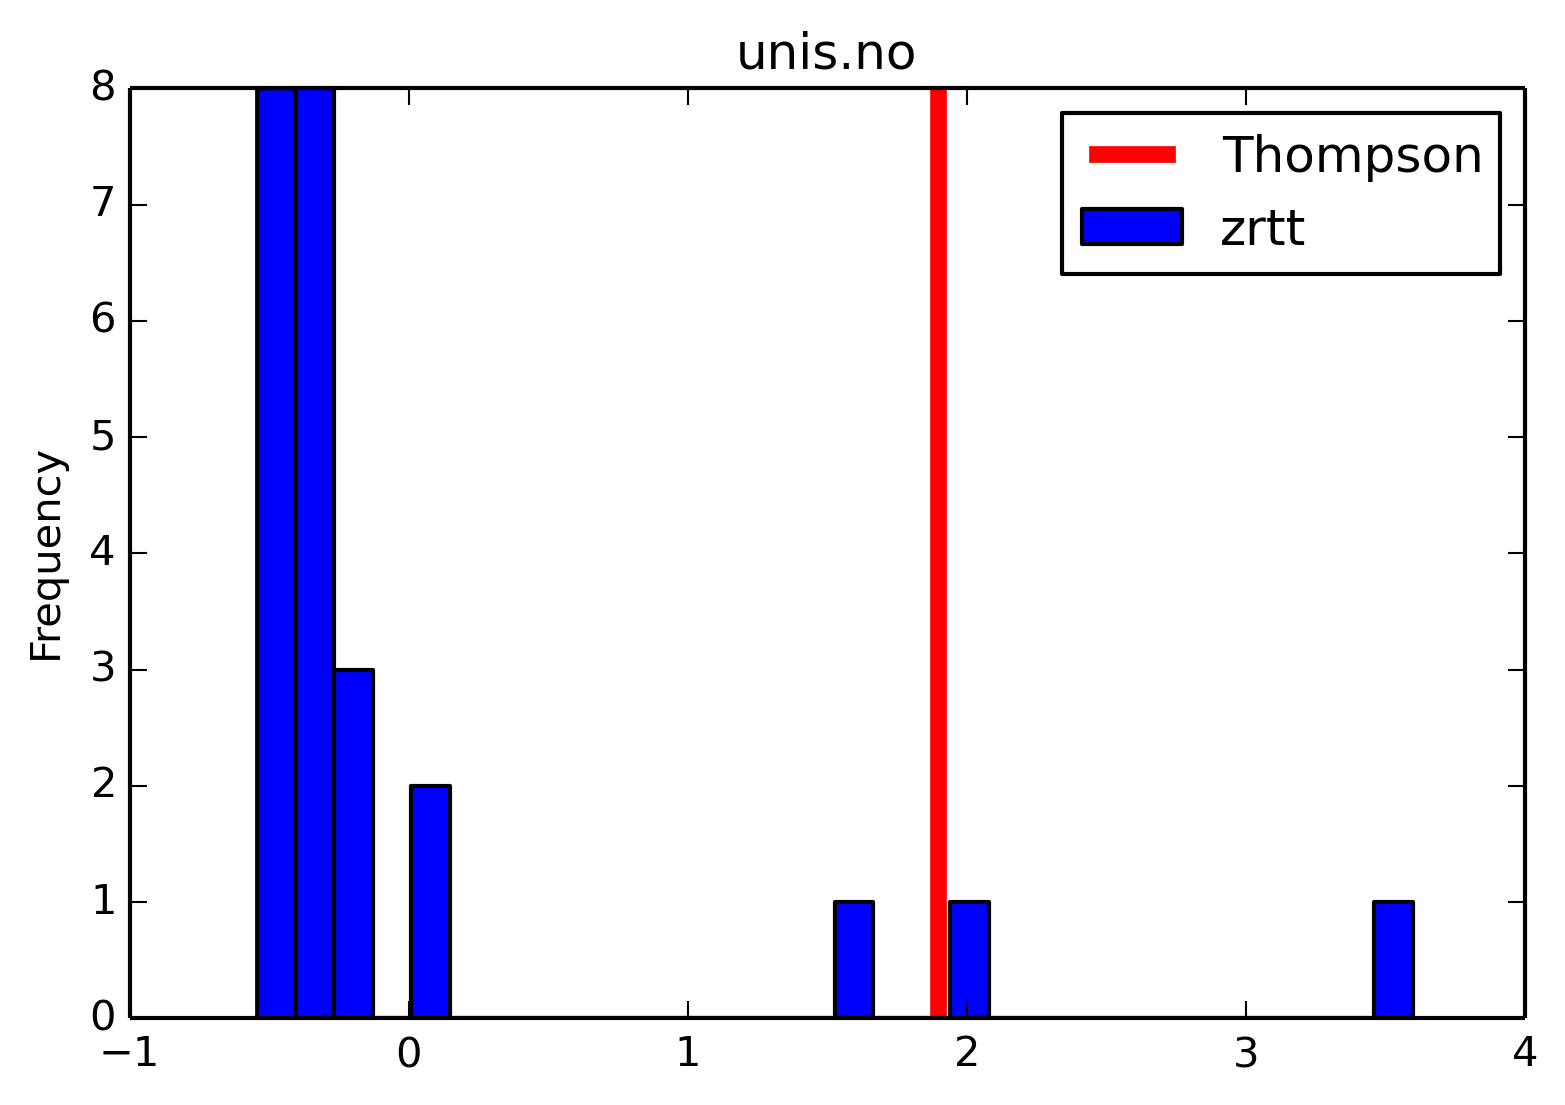
\includegraphics[width=0.45\textwidth]{histogramas_thompson/unis-no.png}
  \caption{RTTs Normailzados comparados con el valor Thompson}
  \label{entropia-s}
\end{figure}

\begin{figure}[H]
  \centering
    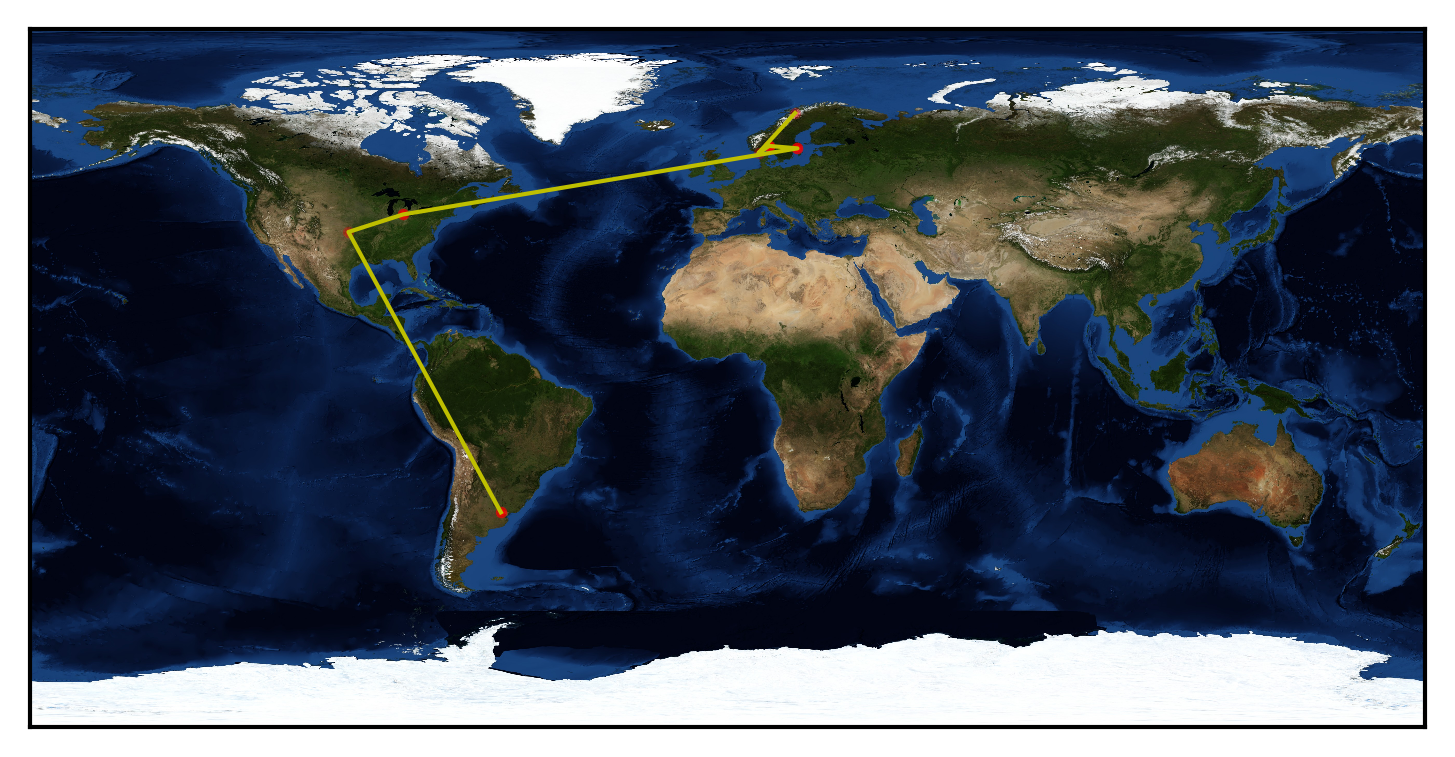
\includegraphics[width=0.45\textwidth]{grafico-rutas/unis-no.png}
  \caption{Gráfico de la ruta}
  \label{entropia-s}
\end{figure}




\subsection{Servidor www.fu-berlin.de}
\begin{center}
\captionof{table}{rtt promedios entre saltos para www.fu-berlin.de}
\begin{tabular}{llllr}
\toprule
                 &    &                &    &       rtt \\
host & ttl & ip & cc &           \\
\midrule
www.fu-berlin.de & 1  & empty & empty &  0.000000 \\
                 & 2  & empty & empty &  0.000000 \\
                 & 3  & empty & empty &  0.000000 \\
                 & 4  & empty & empty &  0.000000 \\
                 & 5  & 200.89.161.97 & AR &  0.076244 \\
                 & 6  & 200.89.165.197 & AR &  0.003247 \\
                 & 7  & 200.89.165.222 & AR &  0.005229 \\
                 & 8  & empty & empty &  0.000000 \\
                 & 9  & 67.17.94.249 & US &  0.131693 \\
                 & 10 & empty & empty &  0.000000 \\
                 & 11 & 4.69.154.73 & DE &  0.093868 \\
                 & 12 & 4.69.154.73 & DE &  0.011529 \\
                 & 13 & 212.162.4.6 & DE &  0.006355 \\
                 & 14 & 188.1.144.134 & DE &  0.014622 \\
                 & 15 & 188.1.234.174 & DE &  0.013845 \\
                 & 16 & 160.45.252.102 & DE &  0.009071 \\
                 & 17 & 130.133.99.102 & DE &  0.001297 \\
                 & 18 & 130.133.99.110 & DE&  0.004726 \\
                 & 19 & 160.45.170.10 & DE &  0.014093 \\
\bottomrule
\end{tabular}

\end{center}

\begin{center}
\begin{tabular}{p{6.5cm}r}
Porcentaje de saltos que no responden los $Time$ $exceeded$: & \textbf{31\%} \\ \\ 
Largo de la ruta en términos de saltos que responden: &\textbf{13 saltos} \\ \\
Cantidad de enlaces intercontinentales: & \textbf{1} \\ \\
Cantidad de outliers según el método de Cimbala: & \textbf{2} \\ \\
\end{tabular}
\end{center}

No se corresponden los enlaces con los outliers.

\begin{figure}[H]
  \centering
    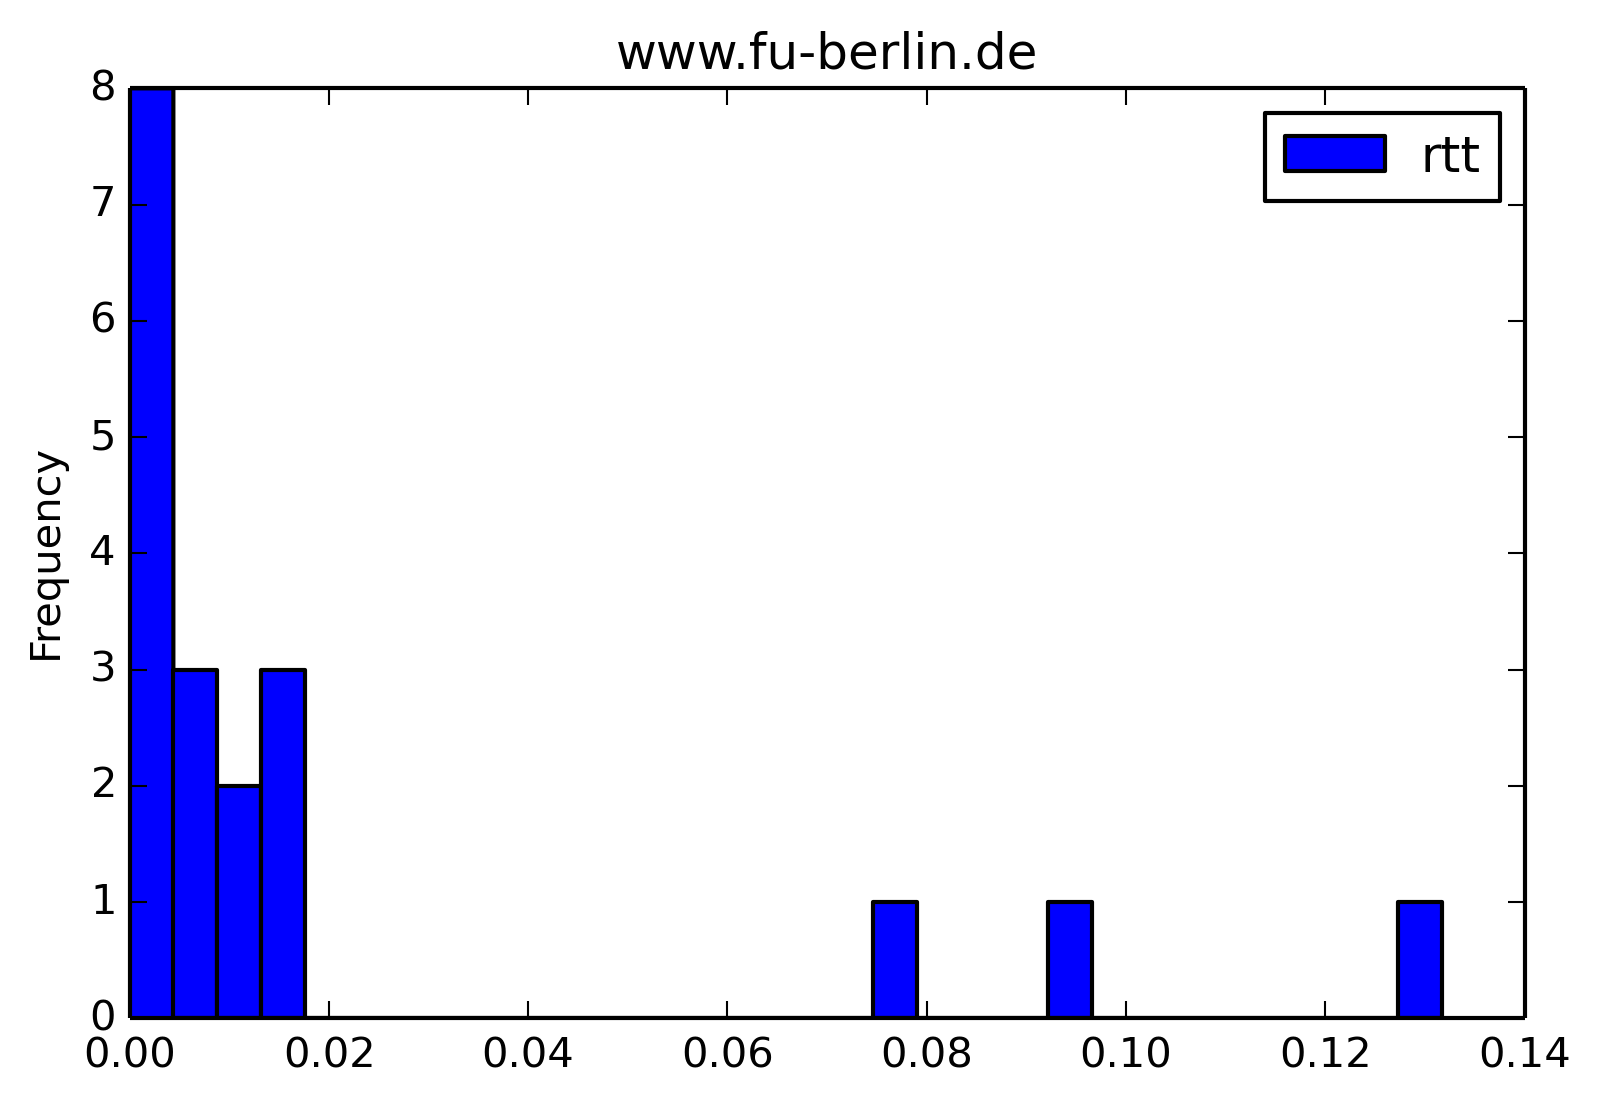
\includegraphics[width=0.45\textwidth]{histogramas_rtt/www-fu-berlin-de.png}
  \caption{RTT entre saltos}
  \label{entropia-s}
\end{figure}

\begin{center}
\captionof{table}{Outliers para www.fu-berlin.de}
\begin{tabular}{llllr}
\toprule
                 &    &                &    &       rtt \\
host & ttl & ip & cc &           \\
\midrule
www.fu-berlin.de & 9  & 67.17.94.249 & US &  2.985575 \\
                 & 11 & 4.69.154.73 &  DE &  1.971715 \\
\bottomrule
\end{tabular}

\end{center}

\begin{figure}[H]
  \centering
    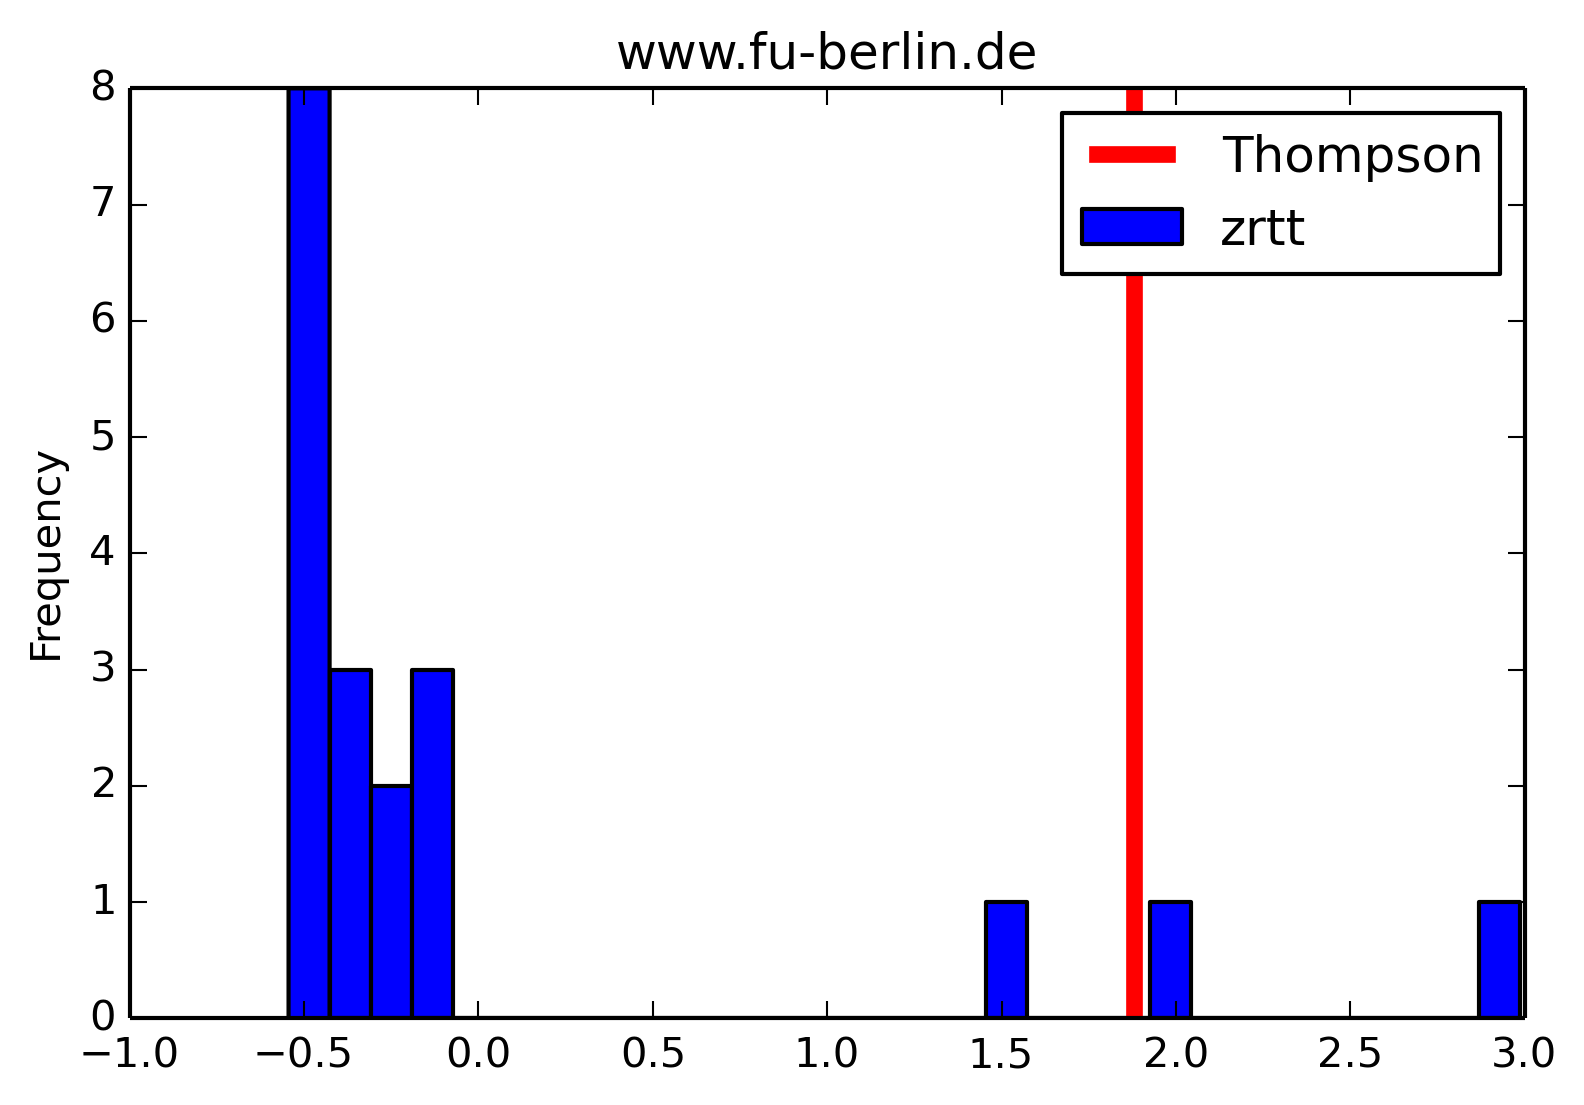
\includegraphics[width=0.45\textwidth]{histogramas_thompson/www-fu-berlin-de.png}
  \caption{RTTs Normailzados comparados con el valor Thompson}
  \label{entropia-s}
\end{figure}

\begin{figure}[H]
  \centering
    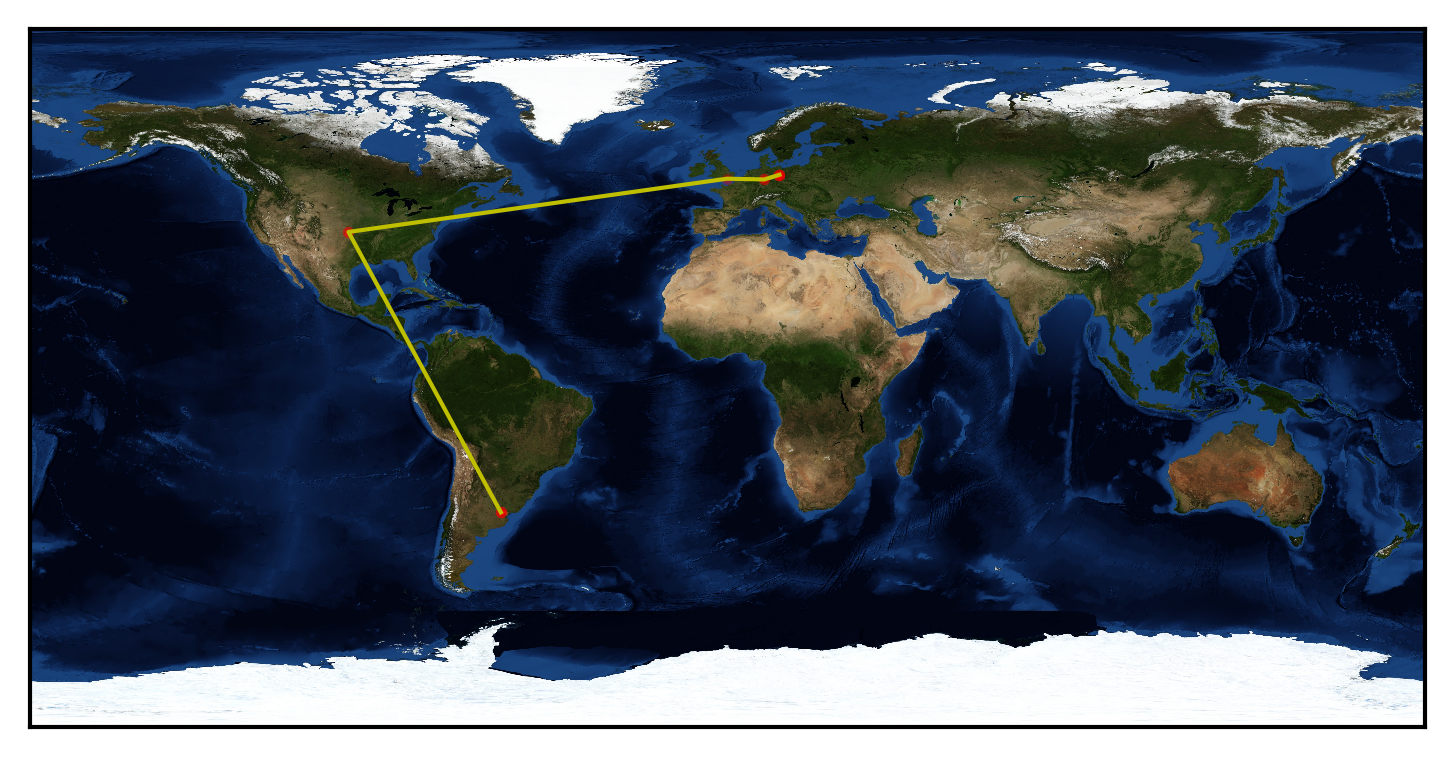
\includegraphics[width=0.45\textwidth]{grafico-rutas/www-fu-berlin-de.png}
  \caption{Gráfico de la ruta}
  \label{entropia-s}
\end{figure}




\subsection{Servidor www.kstu.kz}

\begin{center}
\begin{tabular}{p{6.5cm}r}
Porcentaje de saltos que no responden los $Time$ $exceeded$: & \textbf{40\%} \\ \\ 
Largo de la ruta en términos de saltos que responden: &\textbf{15 saltos} \\ \\
Cantidad de enlaces intercontinentales: & \textbf{1} \\ \\
Cantidad de outliers según el método de Cimbala: & \textbf{1} \\ \\
\end{tabular}
\end{center}


\begin{figure}[H]
  \centering
    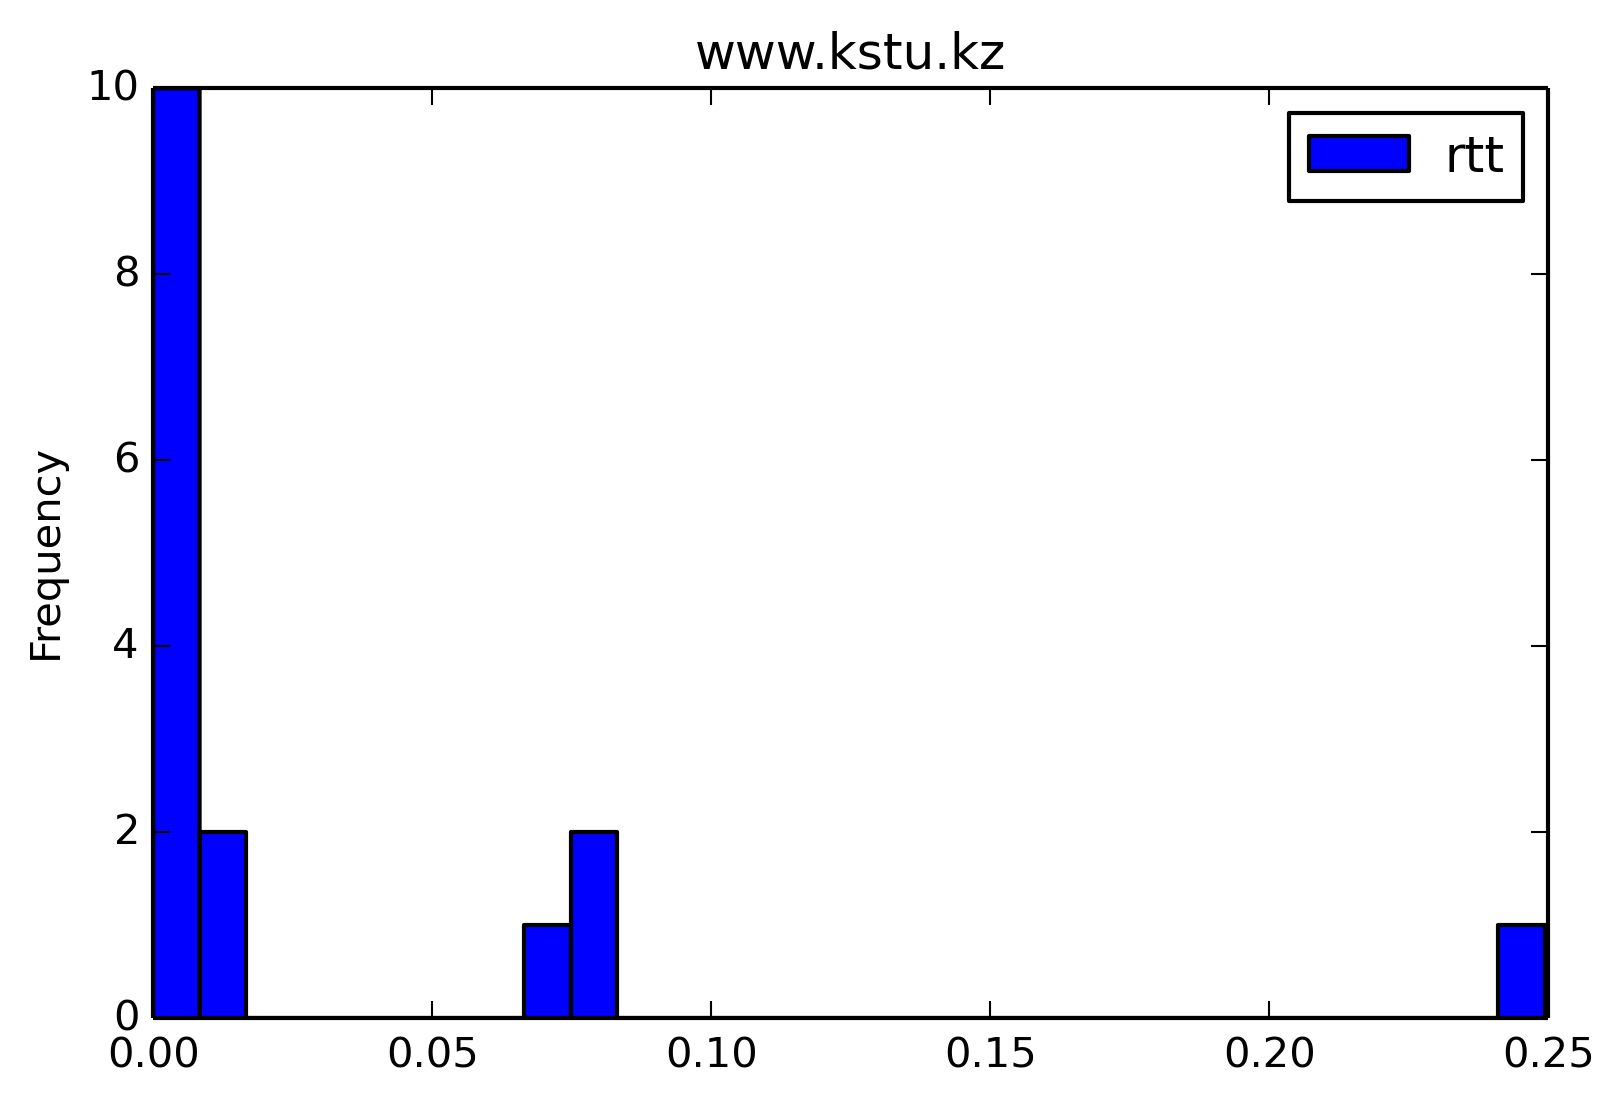
\includegraphics[width=0.45\textwidth]{histogramas_rtt/www-kstu-kz.png}
  \caption{RTT entre saltos}
  \label{entropia-s}
\end{figure}

\begin{figure}[H]
  \centering
    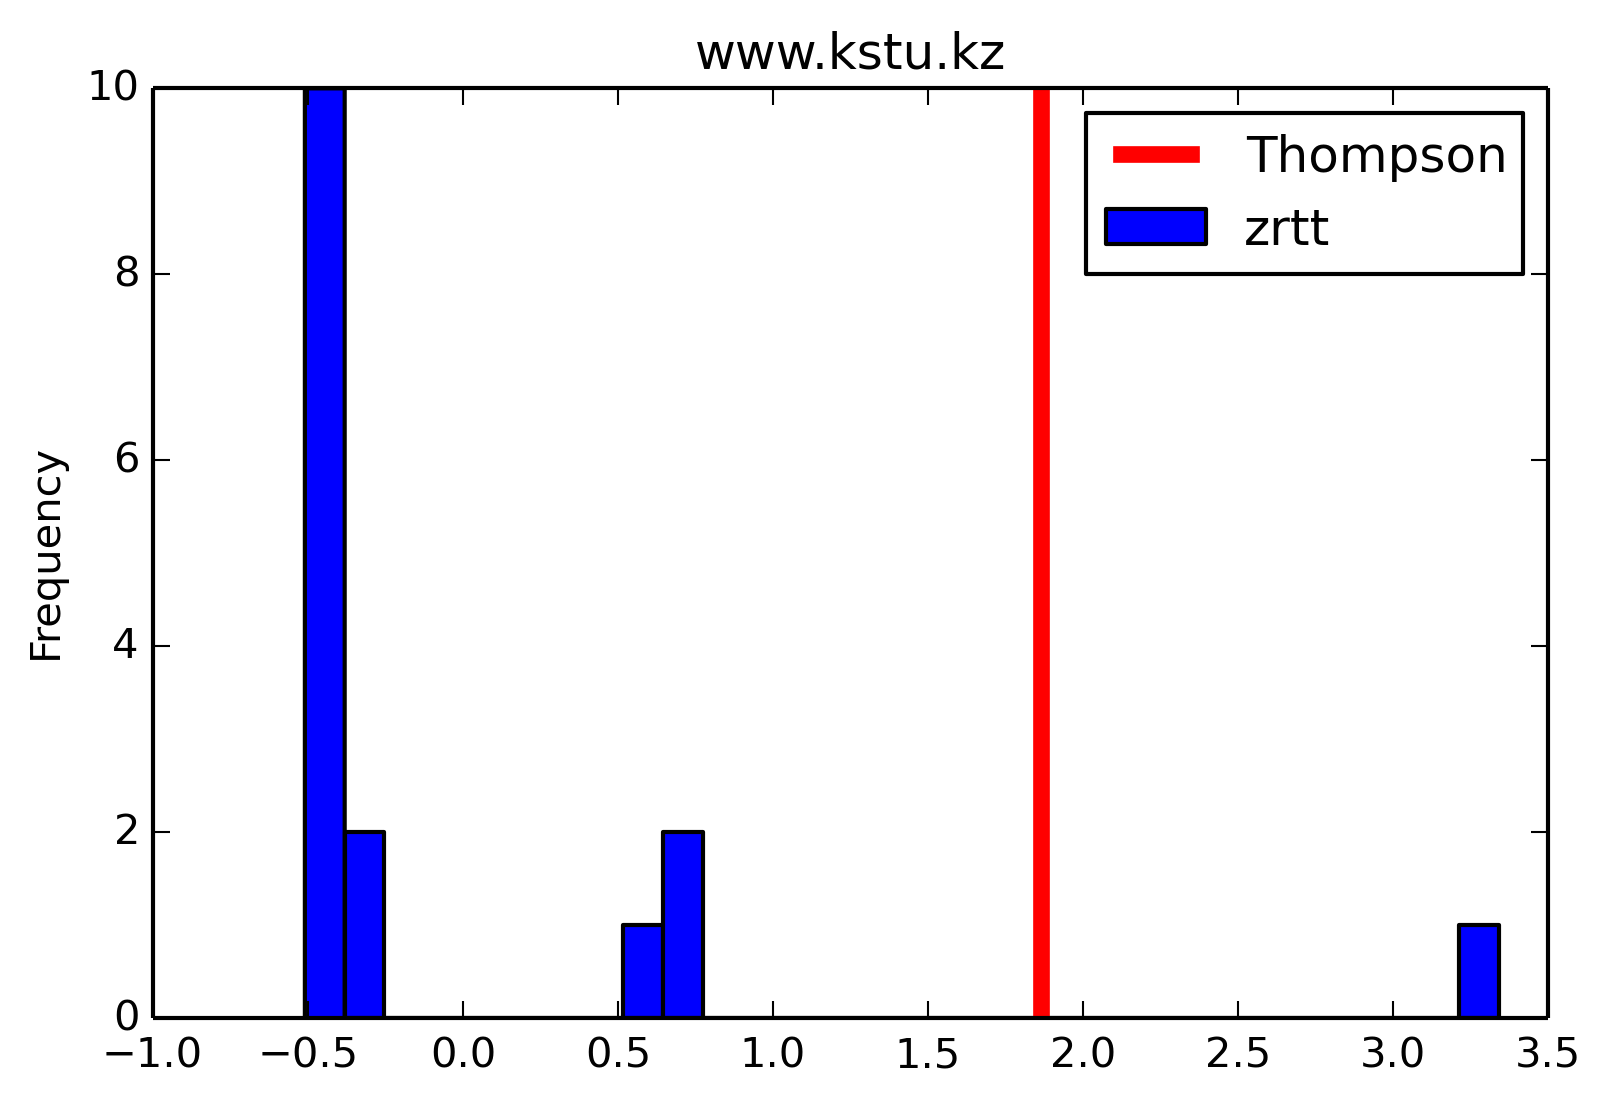
\includegraphics[width=0.45\textwidth]{histogramas_thompson/www-kstu-kz.png}
  \caption{RTTs Normailzados comparados con el valor Thompson}
  \label{entropia-s}
\end{figure}

\begin{figure}[H]
  \centering
    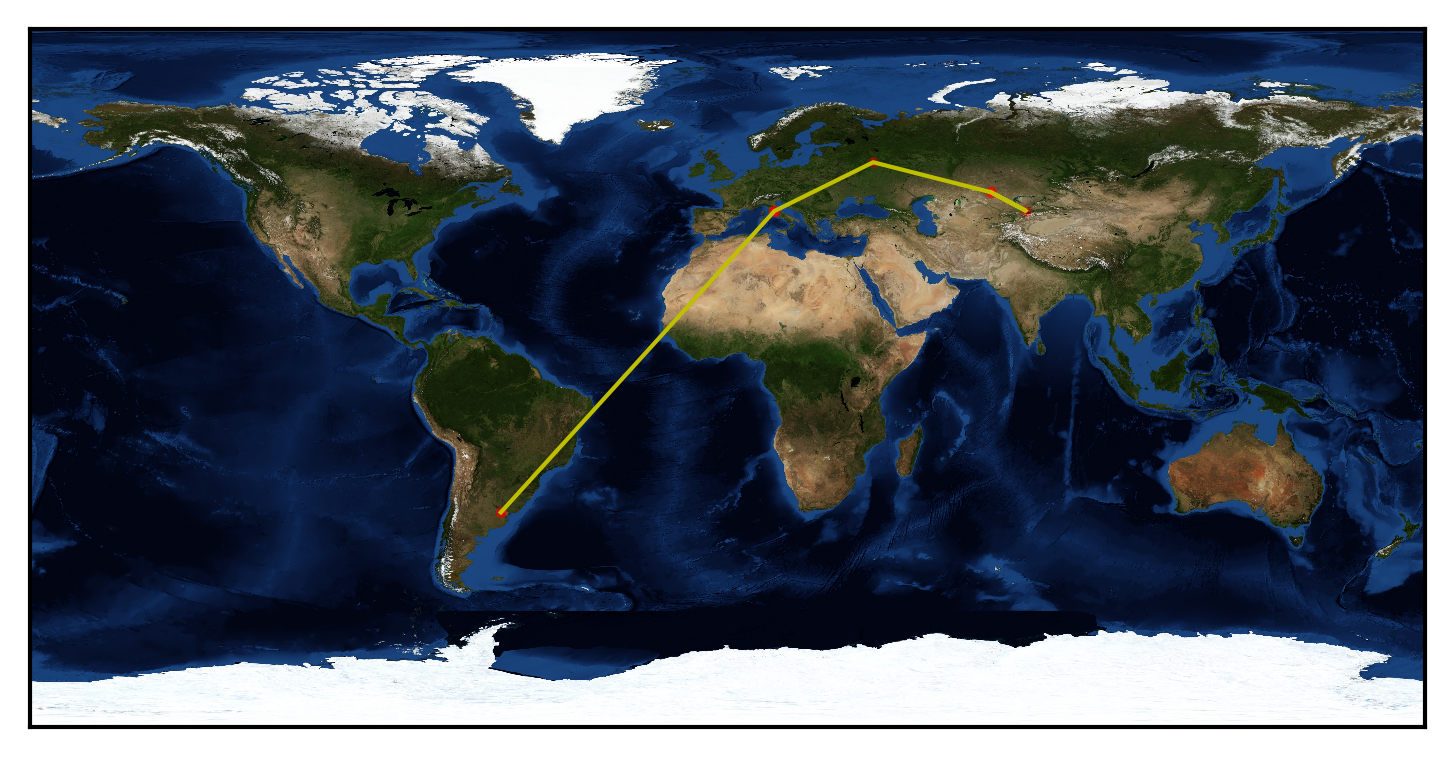
\includegraphics[width=0.45\textwidth]{grafico-rutas/www-kstu-kz.png}
  \caption{Gráfico de la ruta}
  \label{entropia-s}
\end{figure}




\subsection{Servidor www.uq.edu.au}

\begin{center}
\begin{tabular}{p{6.5cm}r}
Porcentaje de saltos que no responden los $Time$ $exceeded$: & \textbf{24\%} \\ \\ 
Largo de la ruta en términos de saltos que responden: &\textbf{22 saltos} \\ \\
Cantidad de enlaces intercontinentales: & \textbf{1} \\ \\
Cantidad de outliers según el método de Cimbala: & \textbf{2} \\ \\
\end{tabular}
\end{center}



\begin{figure}[H]
  \centering
    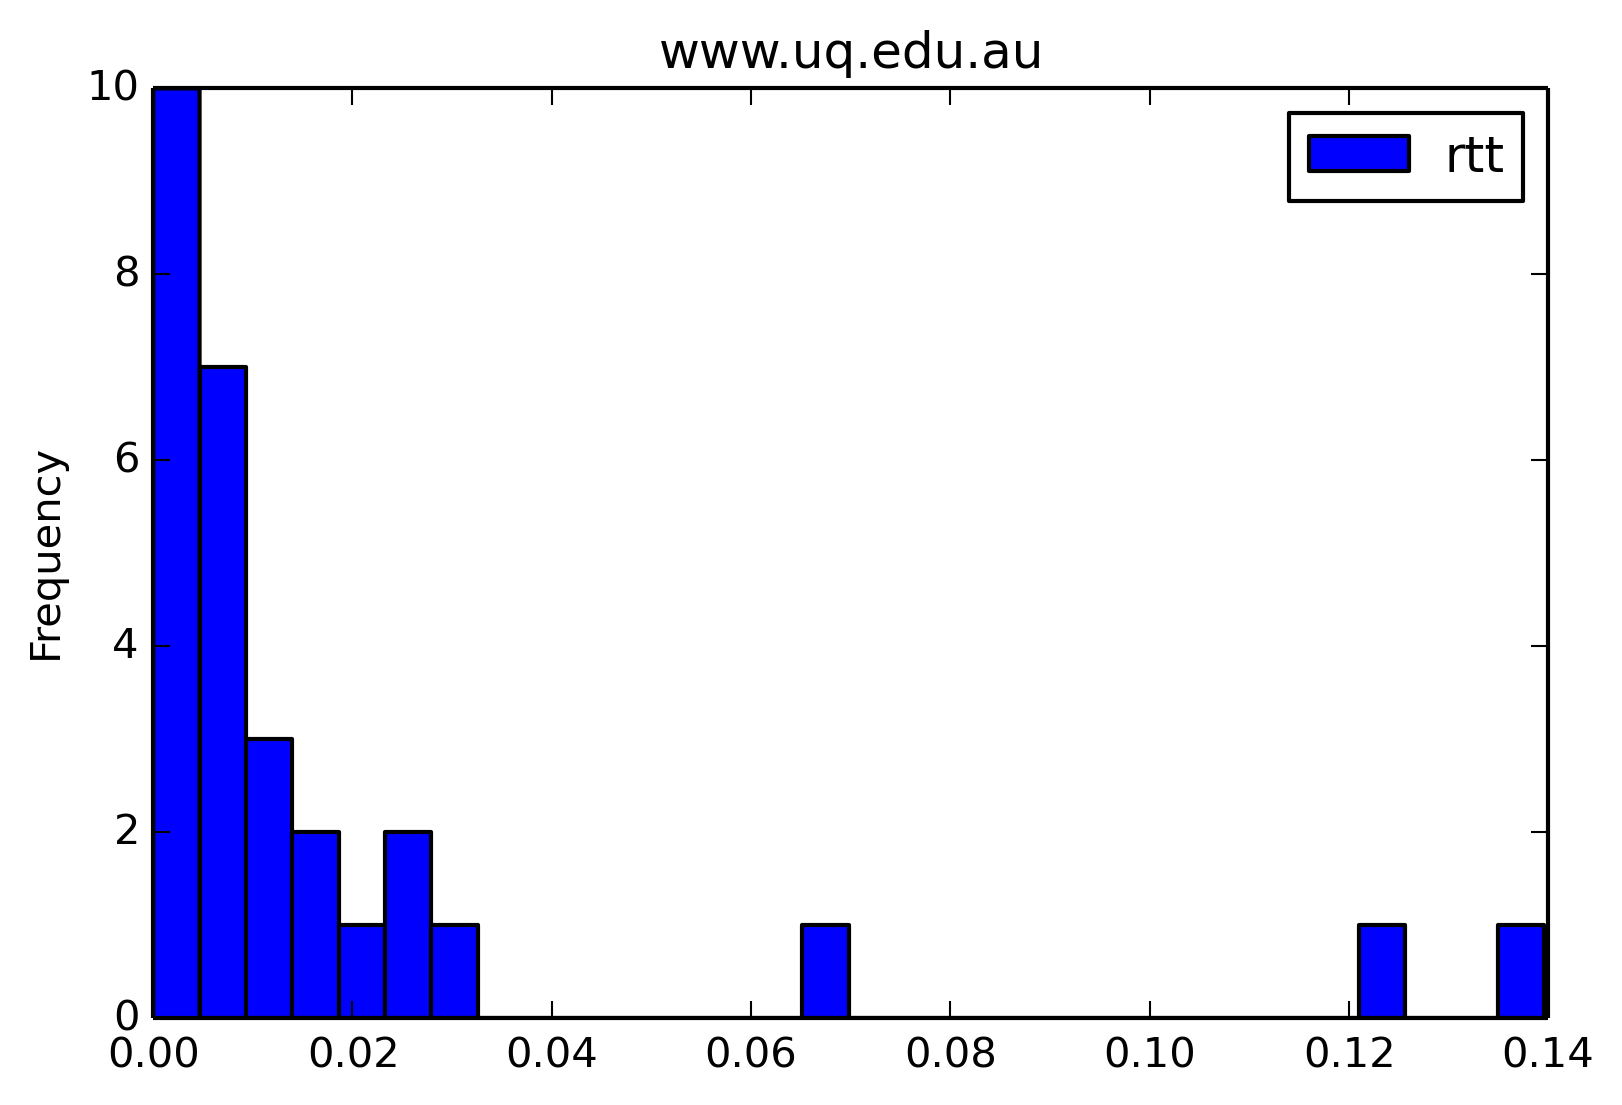
\includegraphics[width=0.45\textwidth]{histogramas_rtt/www-uq-edu-au.png}
  \caption{RTT entre saltos}
  \label{entropia-s}
\end{figure}

\begin{figure}[H]
  \centering
    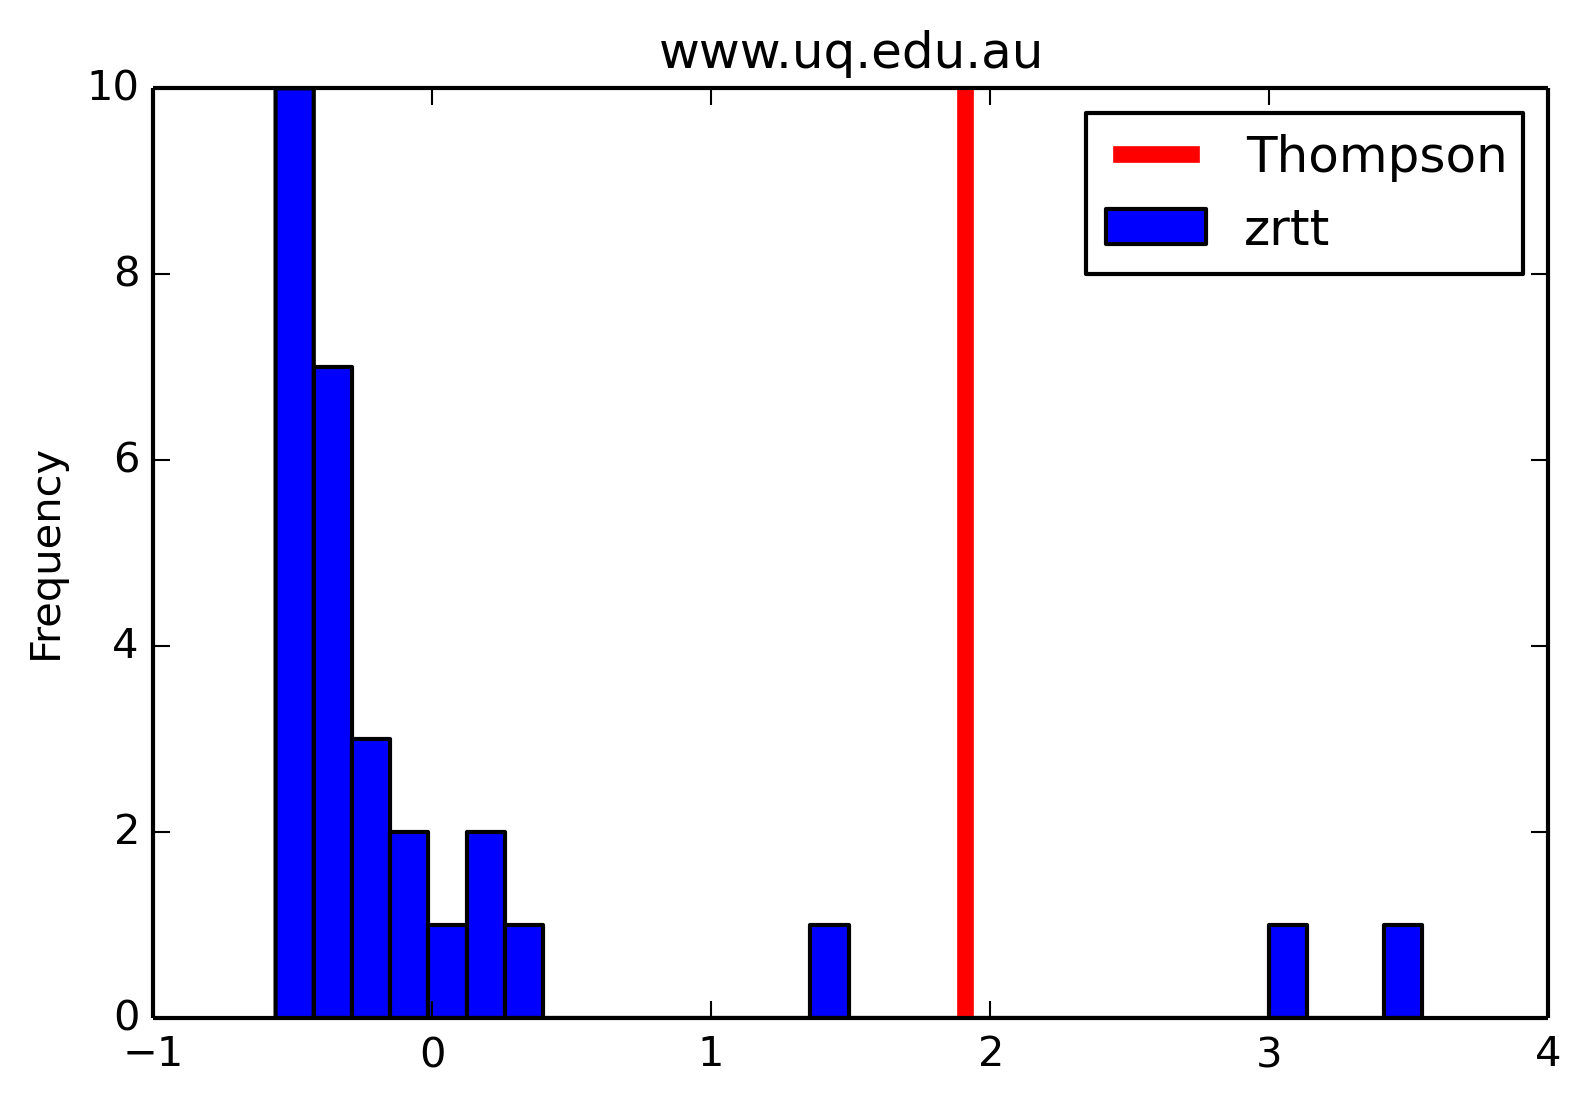
\includegraphics[width=0.45\textwidth]{histogramas_thompson/www-uq-edu-au.png}
  \caption{RTTs Normailzados comparados con el valor Thompson}
  \label{entropia-s}
\end{figure}

\begin{figure}[H]
  \centering
    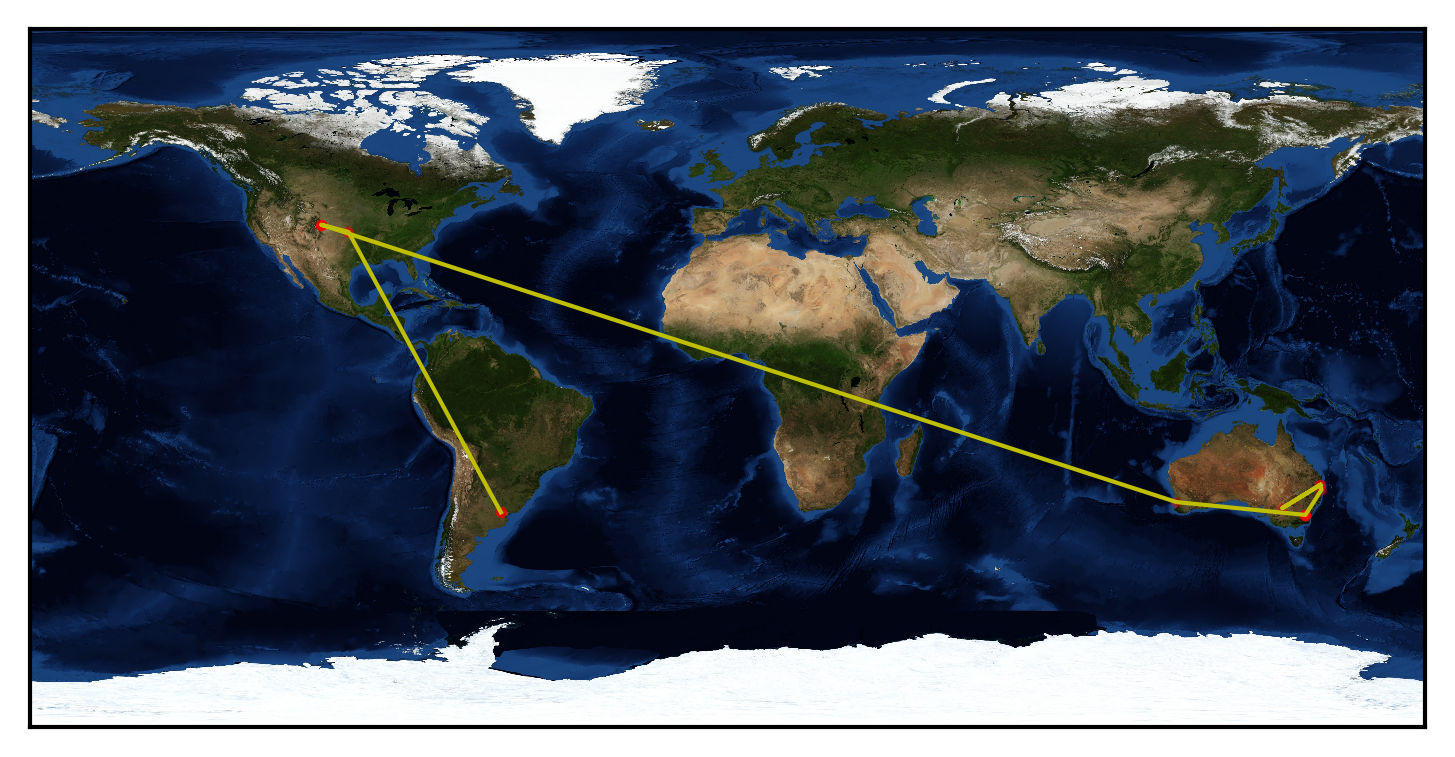
\includegraphics[width=0.45\textwidth]{grafico-rutas/www-uq-edu-au.png}
  \caption{Gráfico de la ruta}
  \label{entropia-s}
\end{figure}





\subsection{Servidor auckland.ac.nz}

\begin{center}
\begin{tabular}{p{6.5cm}r}
Porcentaje de saltos que no responden los $Time$ $exceeded$: & \textbf{\%} \\ \\ 
Largo de la ruta en términos de saltos que responden: &\textbf{ saltos} \\ \\
Cantidad de enlaces intercontinentales: & \textbf{} \\ \\
Cantidad de outliers según el método de Cimbala: & \textbf{} \\ \\
\end{tabular}
\end{center}

\begin{figure}[H]
  \centering
    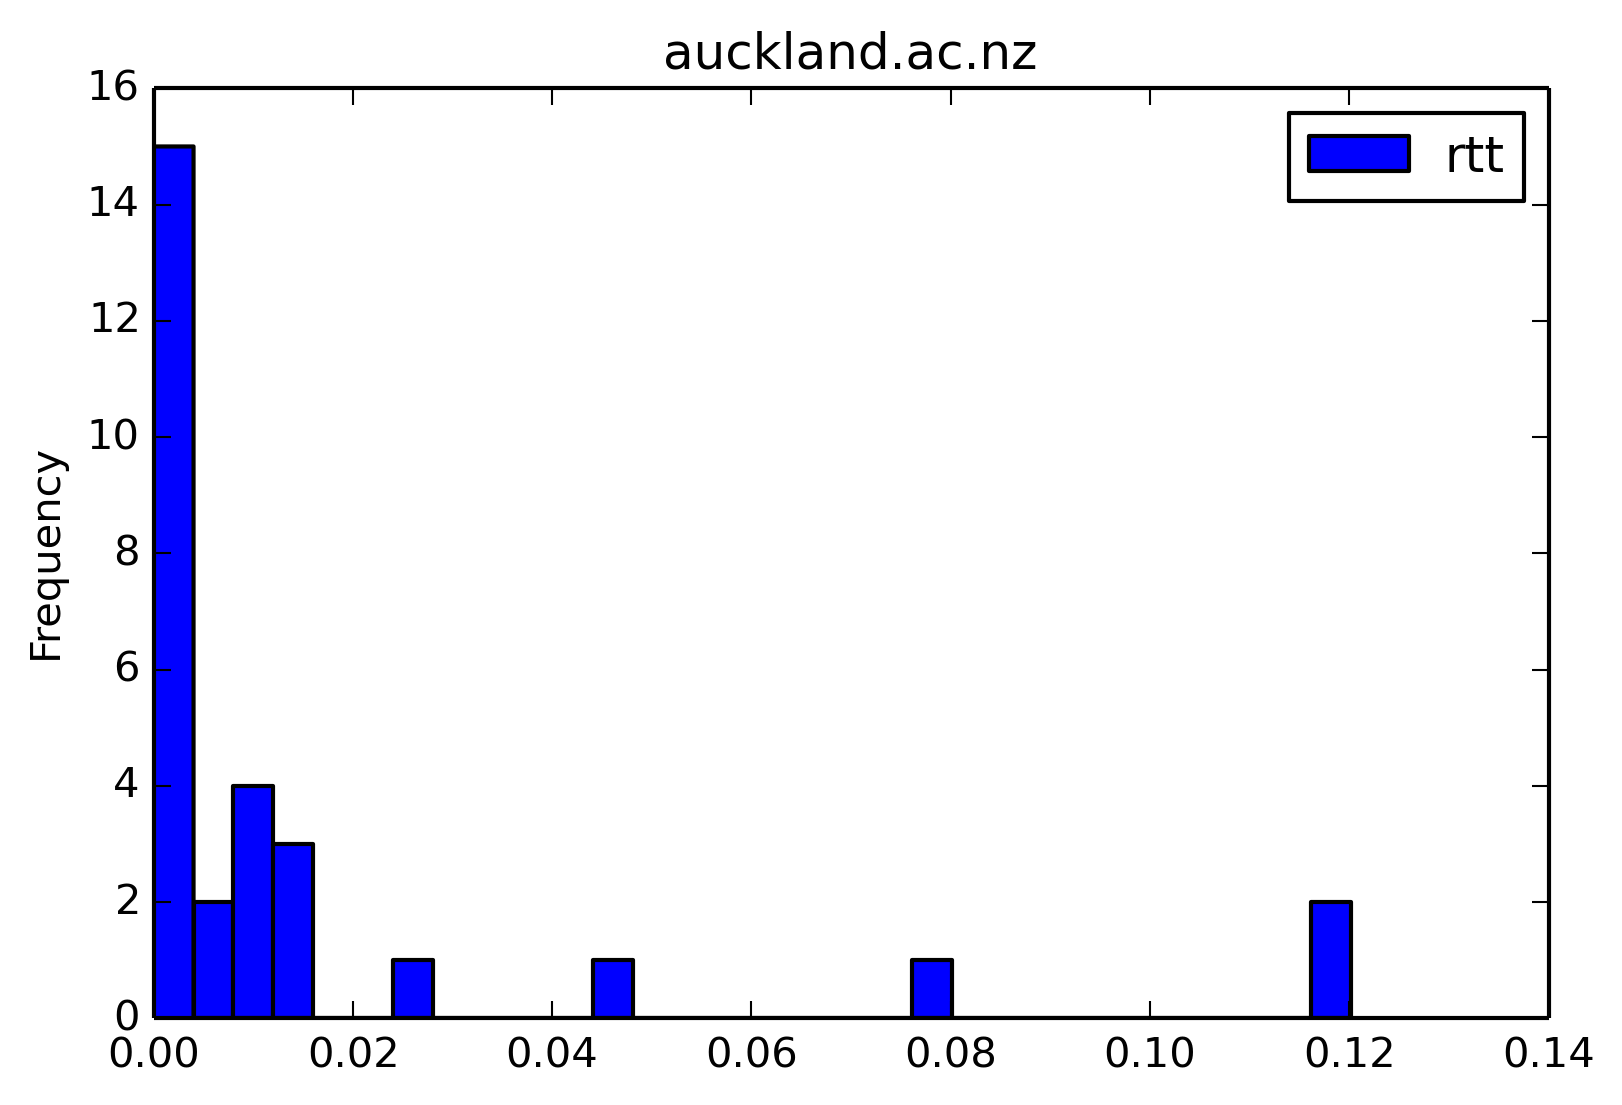
\includegraphics[width=0.45\textwidth]{histogramas_rtt/auckland-ac-nz.png}
  \caption{RTT entre saltos}
  \label{entropia-s}
\end{figure}

\begin{figure}[H]
  \centering
    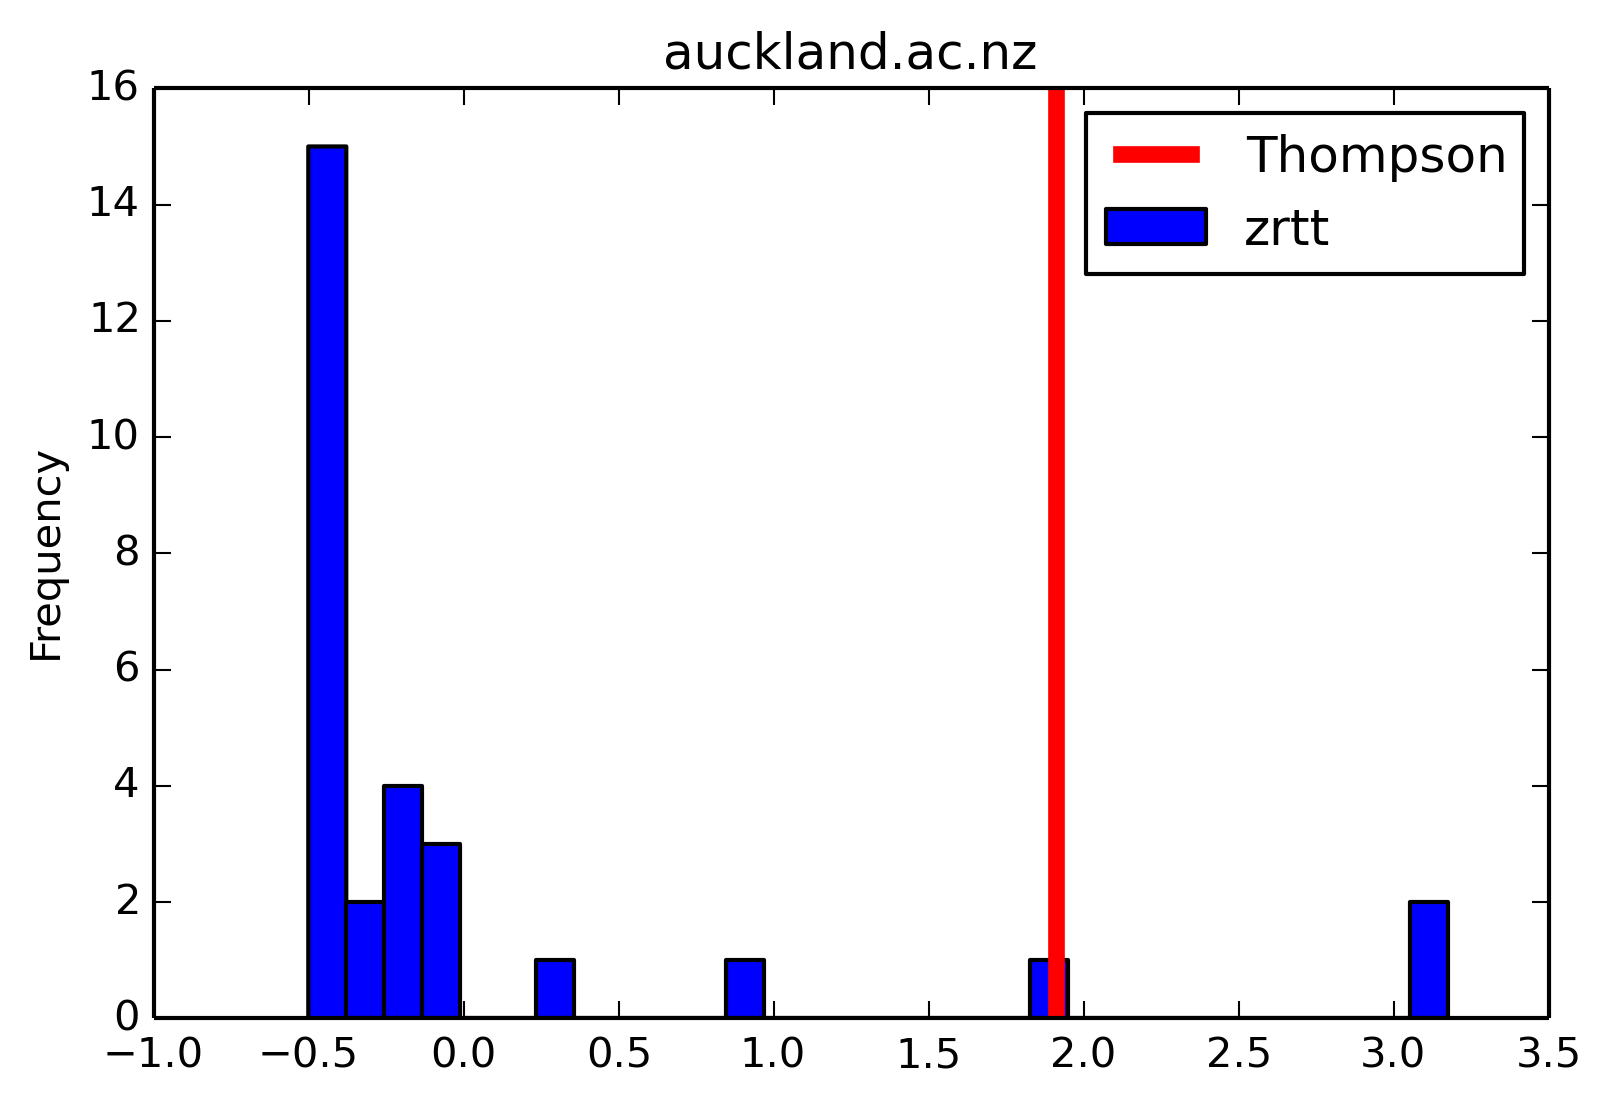
\includegraphics[width=0.45\textwidth]{histogramas_thompson/auckland-ac-nz.png}
  \caption{RTTs Normalizados comparados con el valor Thompson}
  \label{entropia-s}
\end{figure}

\begin{figure}[H]
  \centering
    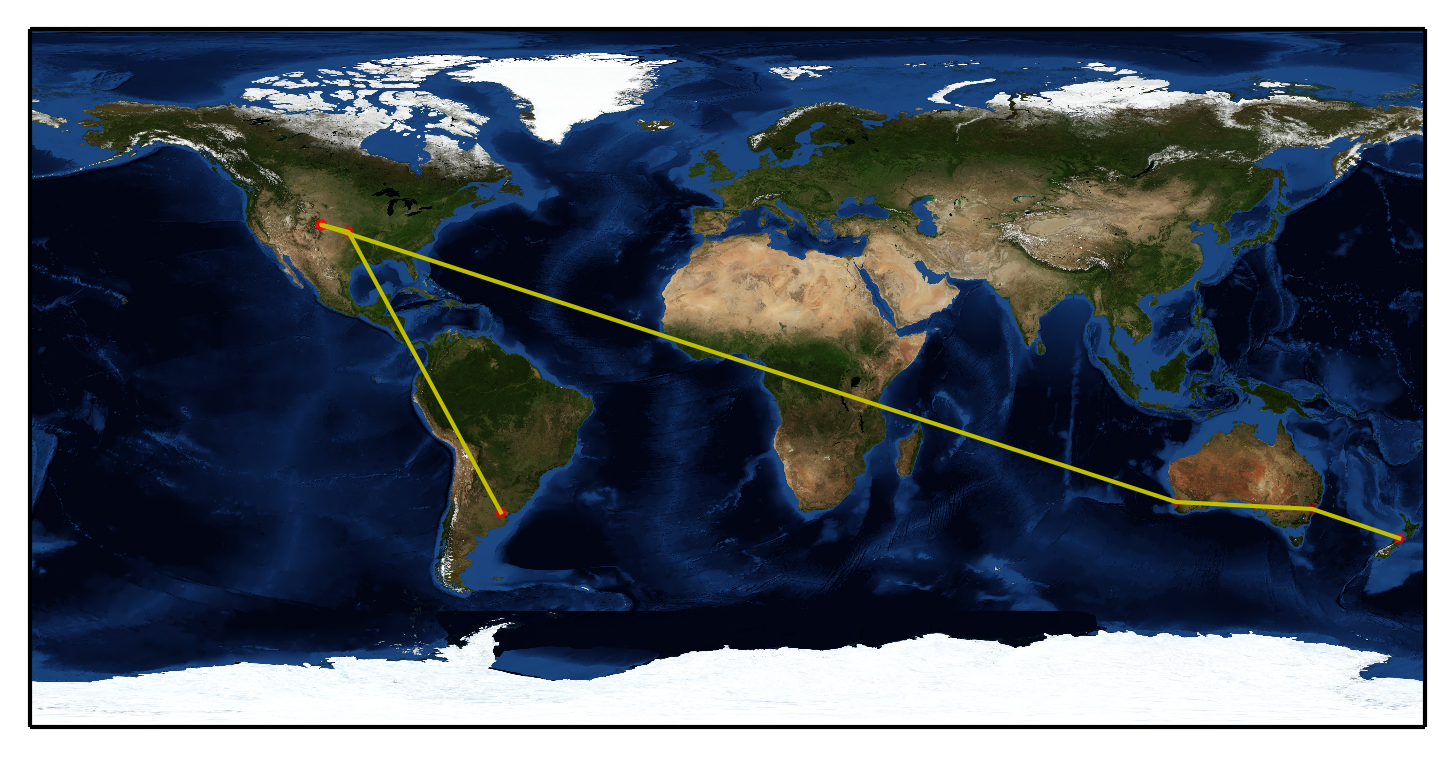
\includegraphics[width=0.45\textwidth]{grafico-rutas/auckland-ac-nz.png}
  \caption{Gráfico de la ruta}
  \label{entropia-s}
\end{figure}




\subsection{Servidor invertisuniversity.ac.in}

\begin{center}
\begin{tabular}{p{6.5cm}r}
Porcentaje de saltos que no responden los $Time$ $exceeded$: & \textbf{\%} \\ \\ 
Largo de la ruta en términos de saltos que responden: &\textbf{ saltos} \\ \\
Cantidad de enlaces intercontinentales: & \textbf{} \\ \\
Cantidad de outliers según el método de Cimbala: & \textbf{} \\ \\
\end{tabular}
\end{center}

\begin{figure}[H]
  \centering
    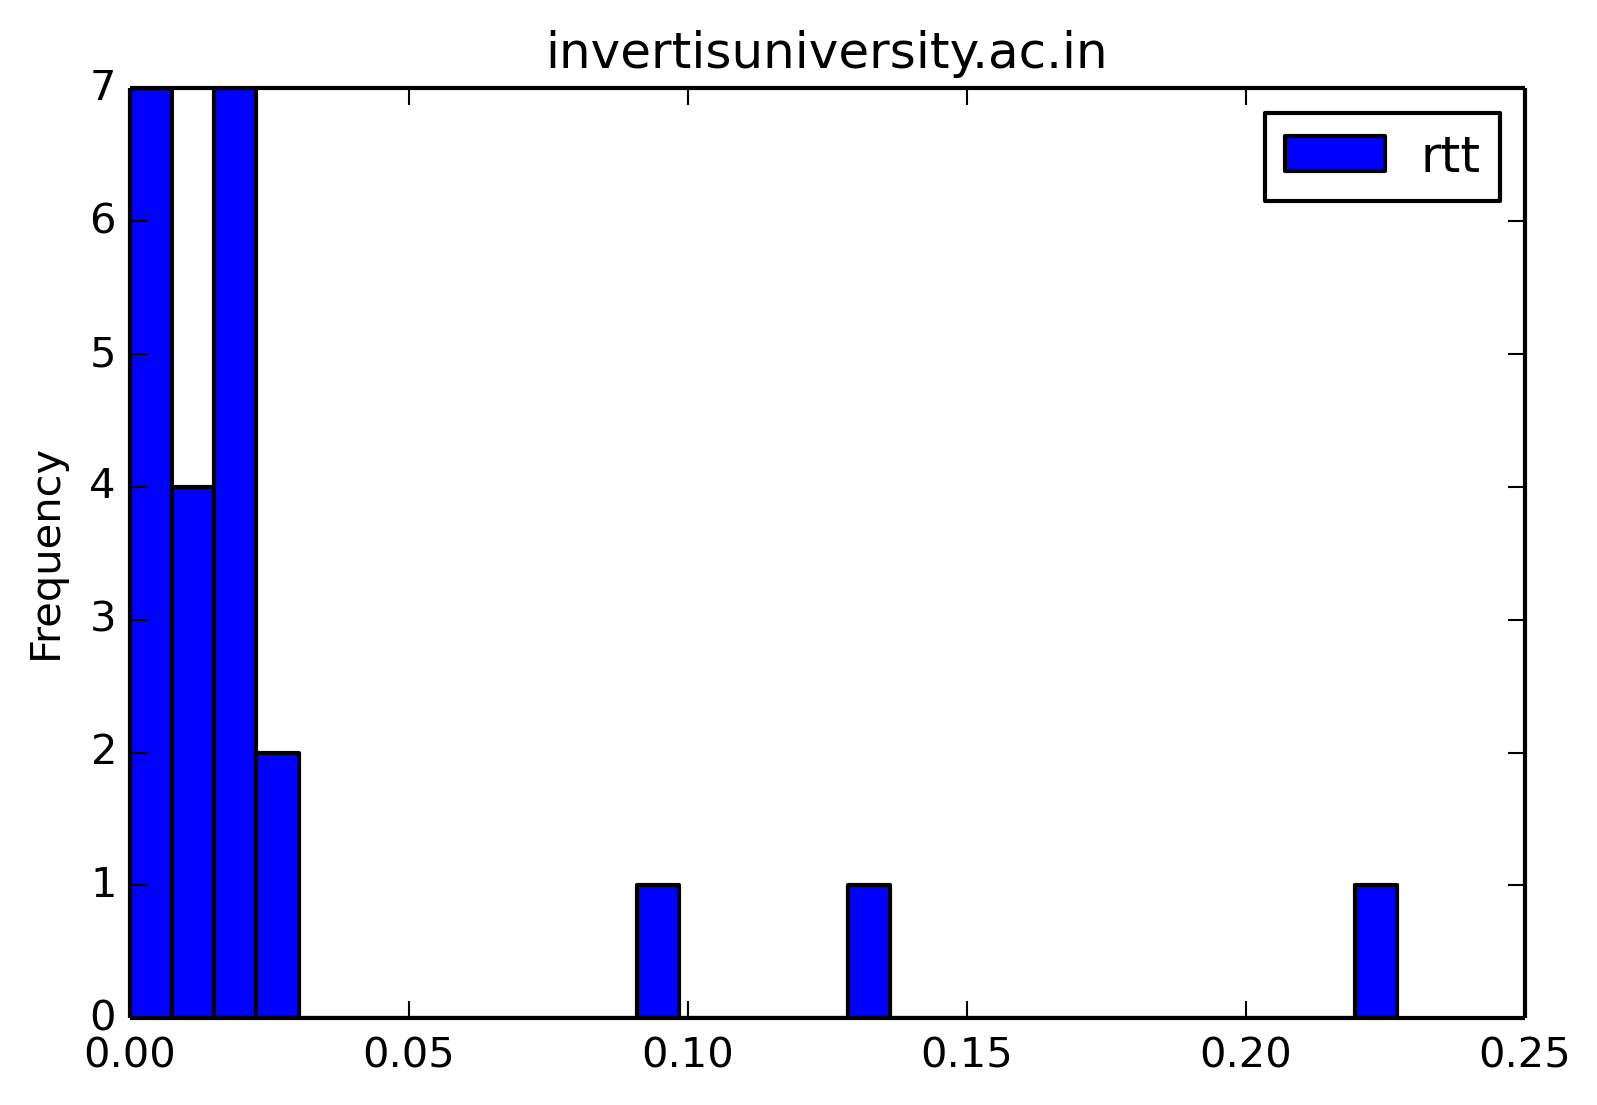
\includegraphics[width=0.45\textwidth]{histogramas_rtt/invertisuniversity-ac-in.png}
  \caption{RTT entre saltos}
  \label{entropia-s}
\end{figure}

\begin{figure}[H]
  \centering
    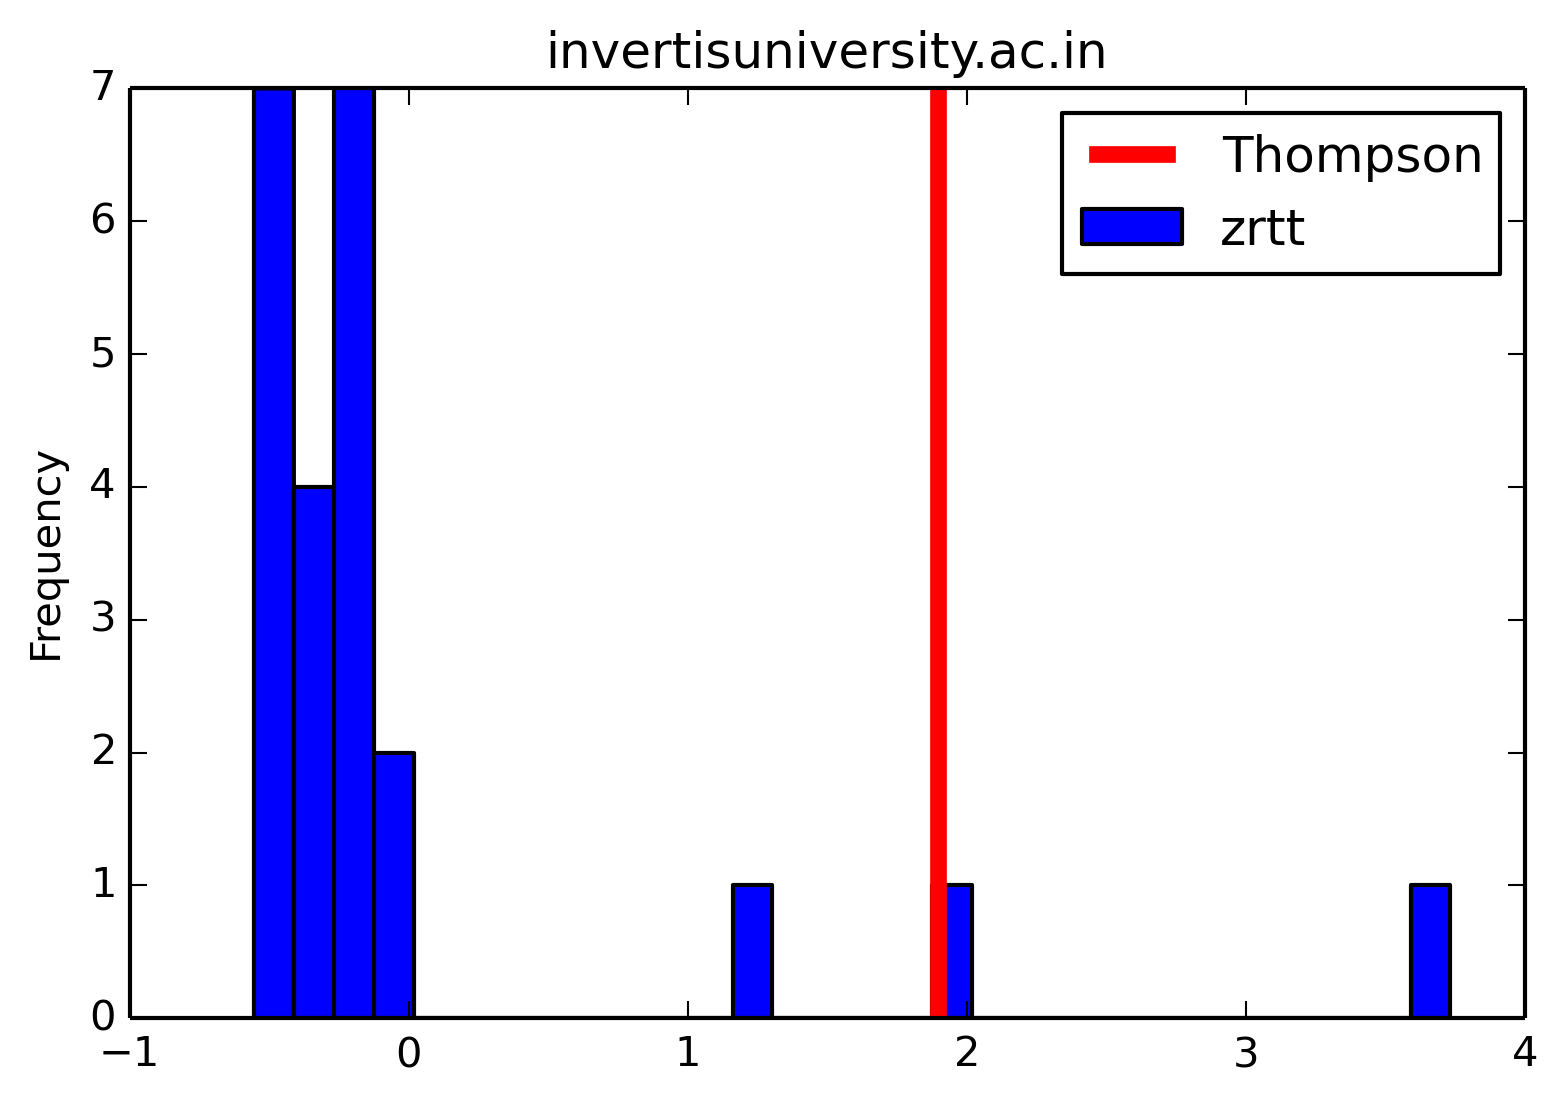
\includegraphics[width=0.45\textwidth]{histogramas_thompson/invertisuniversity-ac-in.png}
  \caption{RTTs Normalizados comparados con el valor Thompson}
  \label{entropia-s}
\end{figure}

\begin{figure}[H]
  \centering
    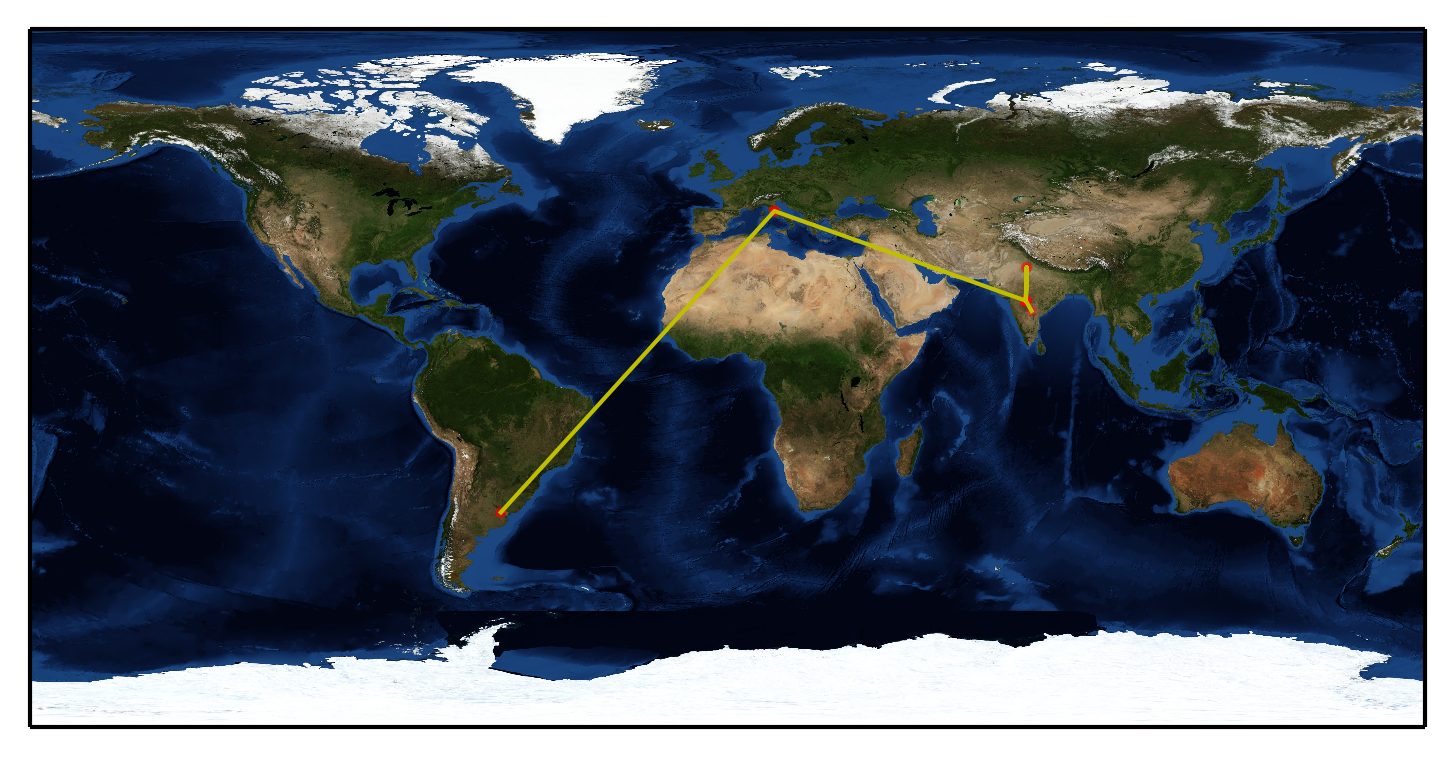
\includegraphics[width=0.45\textwidth]{grafico-rutas/invertisuniversity-ac-in.png}
  \caption{Gráfico de la ruta}
  \label{entropia-s}
\end{figure}




\subsection{Servidor www.uae.ma}

\begin{center}
\begin{tabular}{p{6.5cm}r}
Porcentaje de saltos que no responden los $Time$ $exceeded$: & \textbf{25\%} \\ \\ 
Largo de la ruta en términos de saltos que responden: &\textbf{15 saltos} \\ \\
Cantidad de enlaces intercontinentales: & \textbf{4} \\ \\
Cantidad de outliers según el método de Cimbala: & \textbf{} \\ \\
\end{tabular}
\end{center}


\begin{figure}[H]
  \centering
    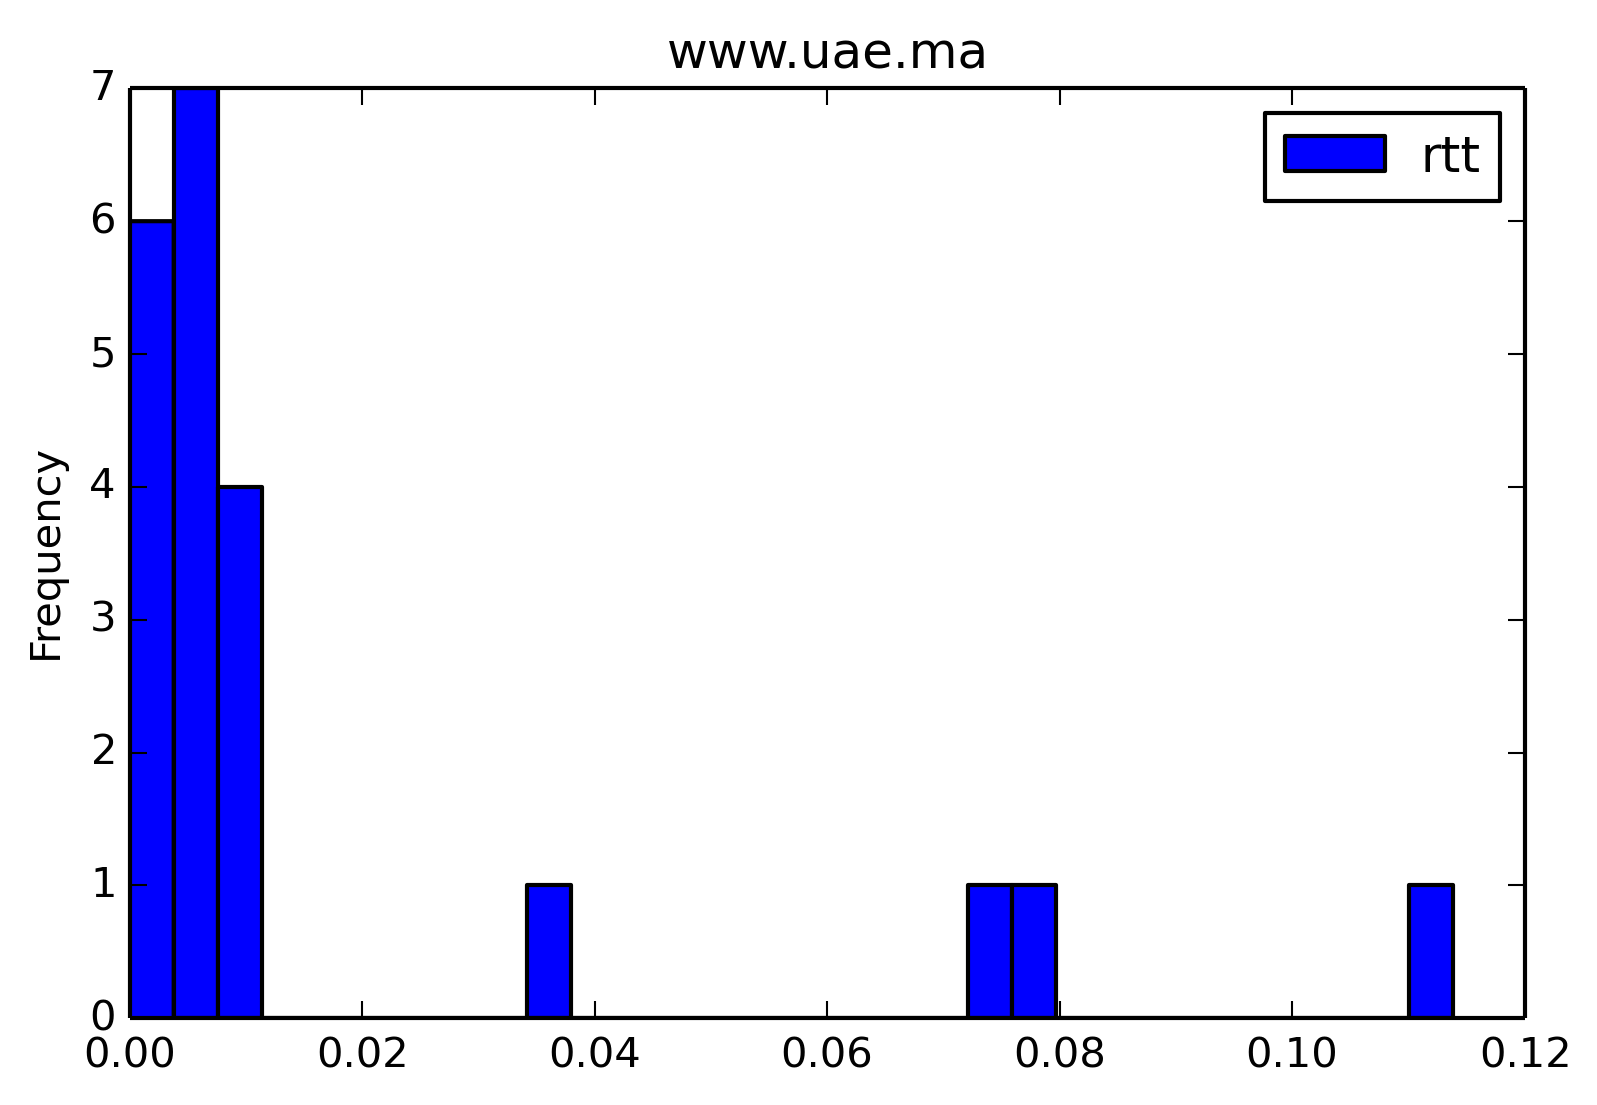
\includegraphics[width=0.45\textwidth]{histogramas_rtt/www-uae-ma.png}
  \caption{RTT entre saltos}
  \label{entropia-s}
\end{figure}

\begin{figure}[H]
  \centering
    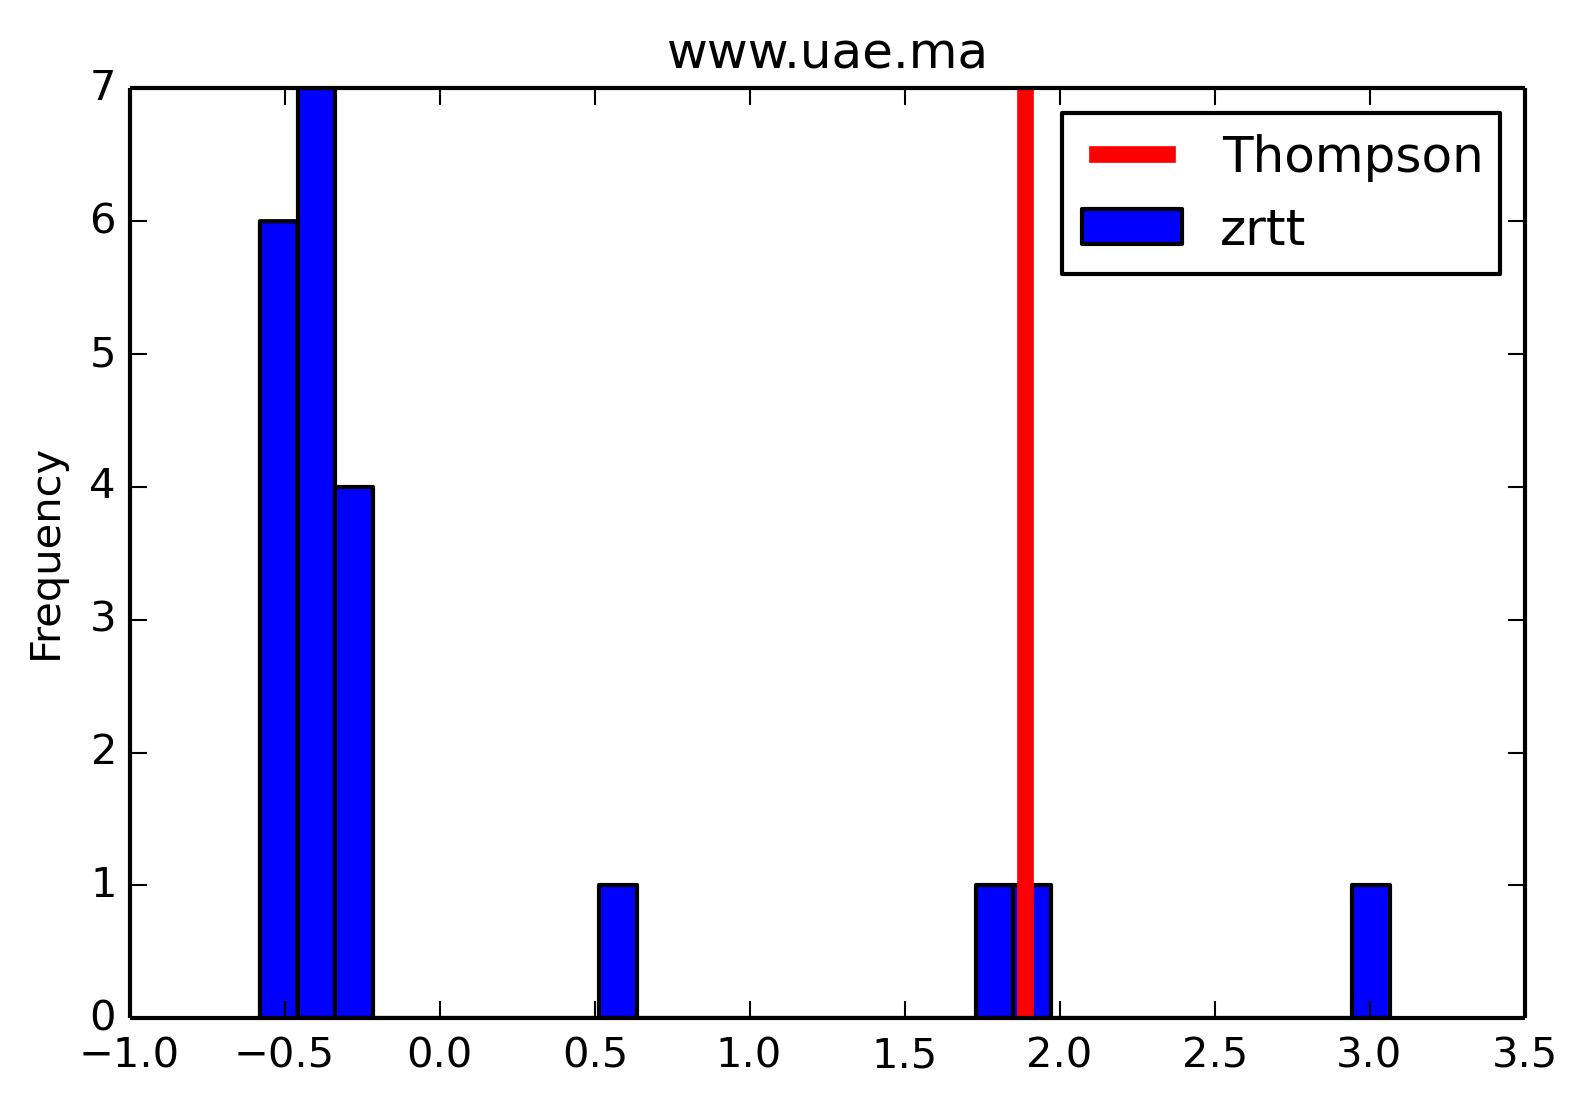
\includegraphics[width=0.45\textwidth]{histogramas_thompson/www-uae-ma.png}
  \caption{RTTs Normalizados comparados con el valor Thompson}
  \label{entropia-s}
\end{figure}

\begin{figure}[H]
  \centering
    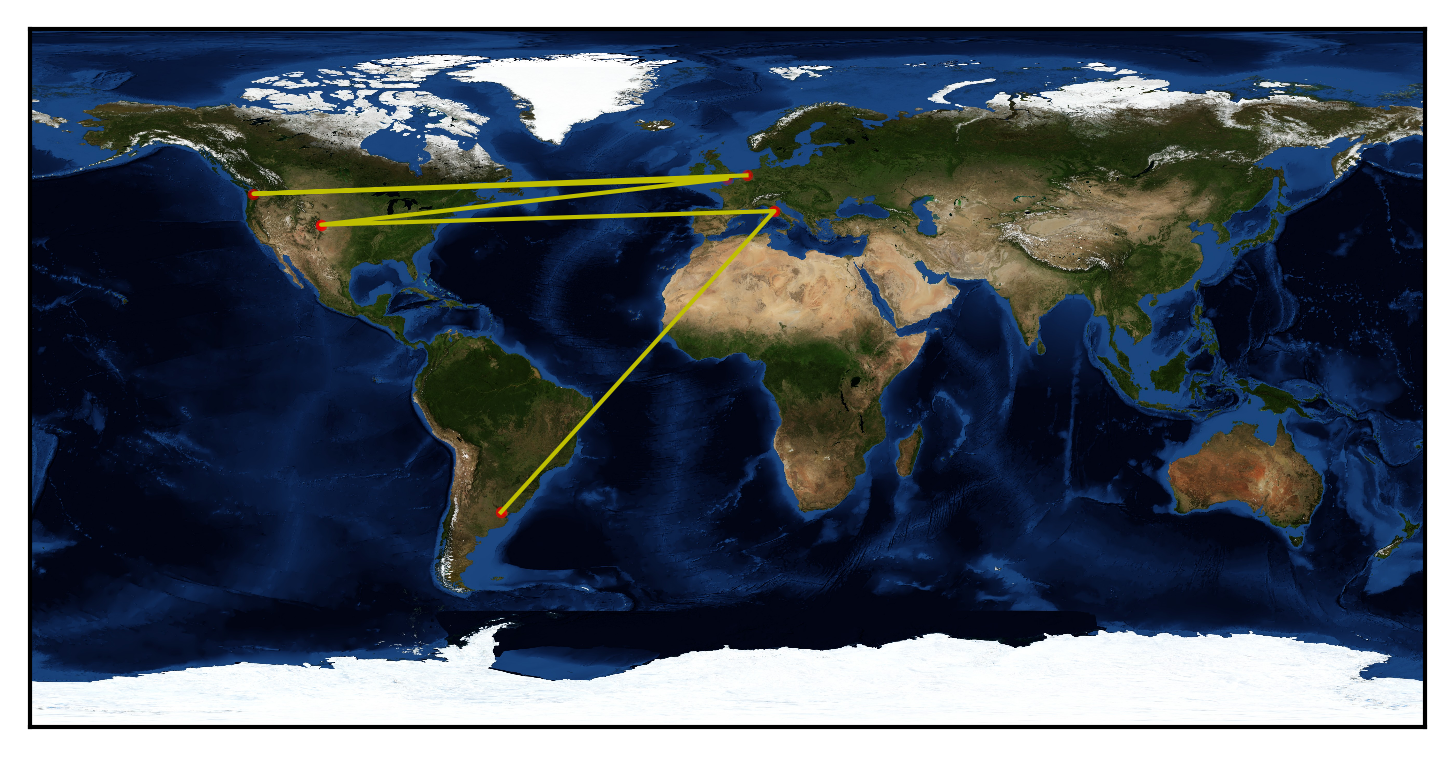
\includegraphics[width=0.45\textwidth]{grafico-rutas/www-uae-ma.png}
  \caption{Gráfico de la ruta}
  \label{entropia-s}
\end{figure}




\subsection{Servidor bifrost.is}

\begin{center}
\begin{tabular}{p{6.5cm}r}
Porcentaje de saltos que no responden los $Time$ $exceeded$: & \textbf{17\%} \\ \\ 
Largo de la ruta en términos de saltos que responden: &\textbf{20 saltos} \\ \\
Cantidad de enlaces intercontinentales: & \textbf{4} \\ \\
Cantidad de outliers según el método de Cimbala: & \textbf{} \\ \\
\end{tabular}
\end{center}

\begin{figure}[H]
  \centering
    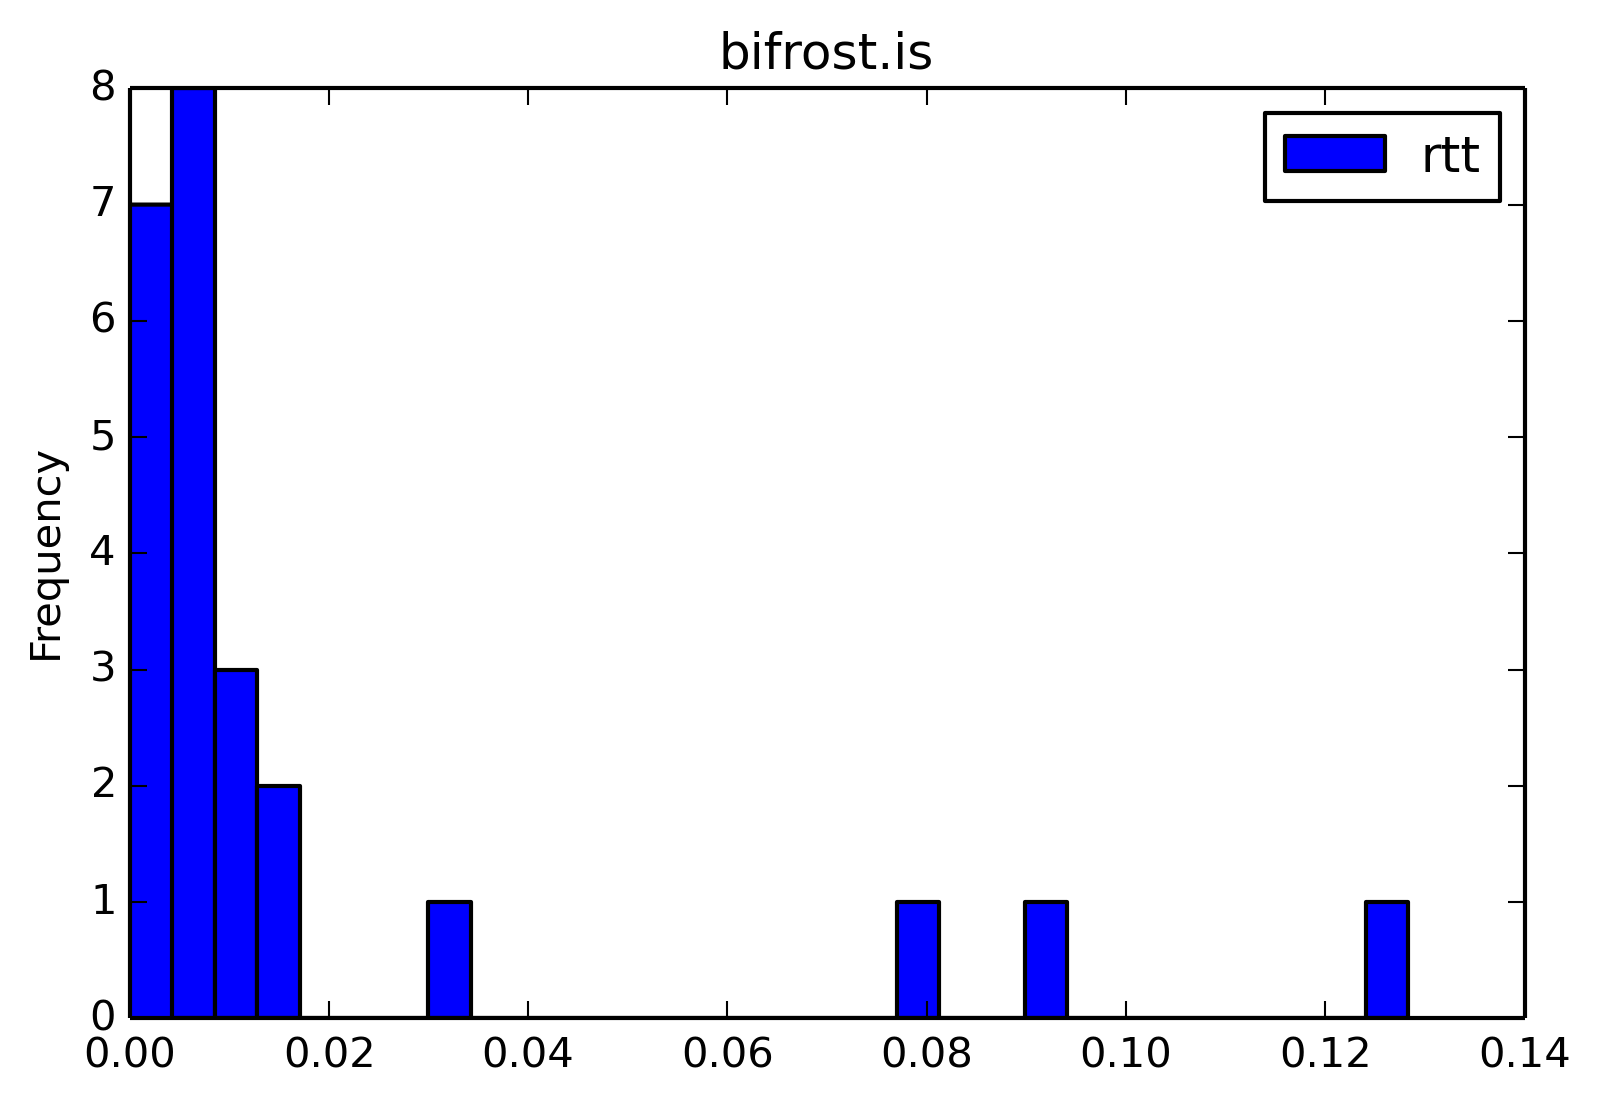
\includegraphics[width=0.45\textwidth]{histogramas_rtt/bifrost-is.png}
  \caption{RTT entre saltos}
  \label{entropia-s}
\end{figure}

\begin{figure}[H]
  \centering
    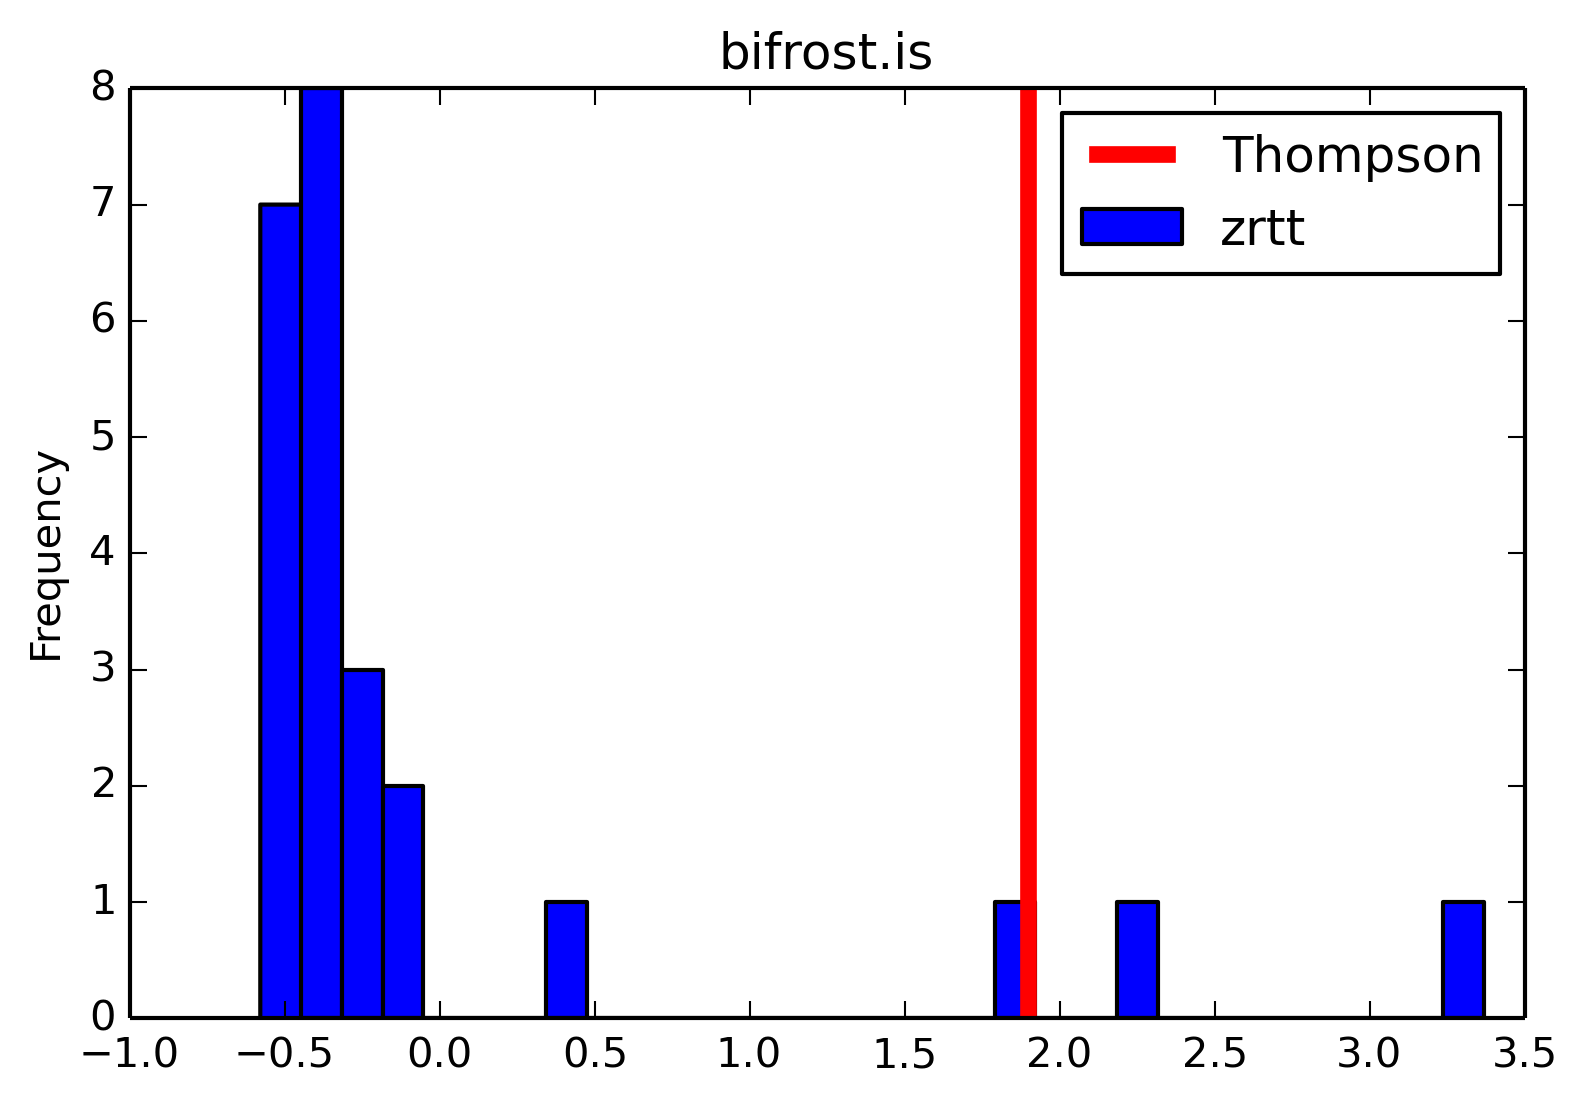
\includegraphics[width=0.45\textwidth]{histogramas_thompson/bifrost-is.png}
  \caption{RTTs Normalizados comparados con el valor Thompson}
  \label{entropia-s}
\end{figure}

\begin{figure}[H]
  \centering
    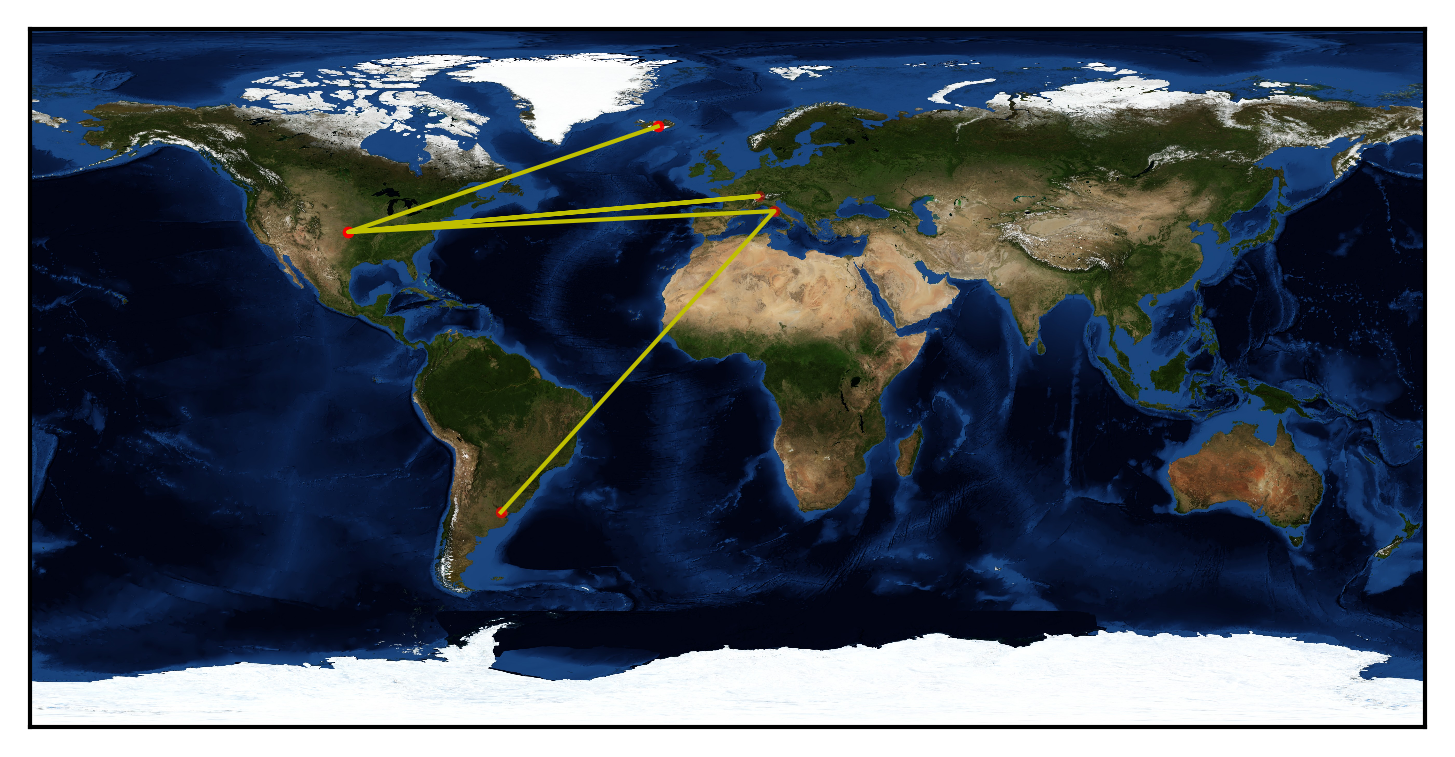
\includegraphics[width=0.45\textwidth]{grafico-rutas/bifrost-is.png}
  \caption{Gráfico de la ruta}
  \label{entropia-s}
\end{figure}




\subsection{Servidor birmingham.ac.uk}

\begin{center}
\begin{tabular}{p{6.5cm}r}
Porcentaje de saltos que no responden los $Time$ $exceeded$: & \textbf{62\%} \\ \\ 
Largo de la ruta en términos de saltos que responden: &\textbf{11 saltos} \\ \\
Cantidad de enlaces intercontinentales: & \textbf{1} \\ \\
Cantidad de outliers según el método de Cimbala: & \textbf{3} \\ \\
\end{tabular}
\end{center}

\begin{figure}[H]
  \centering
    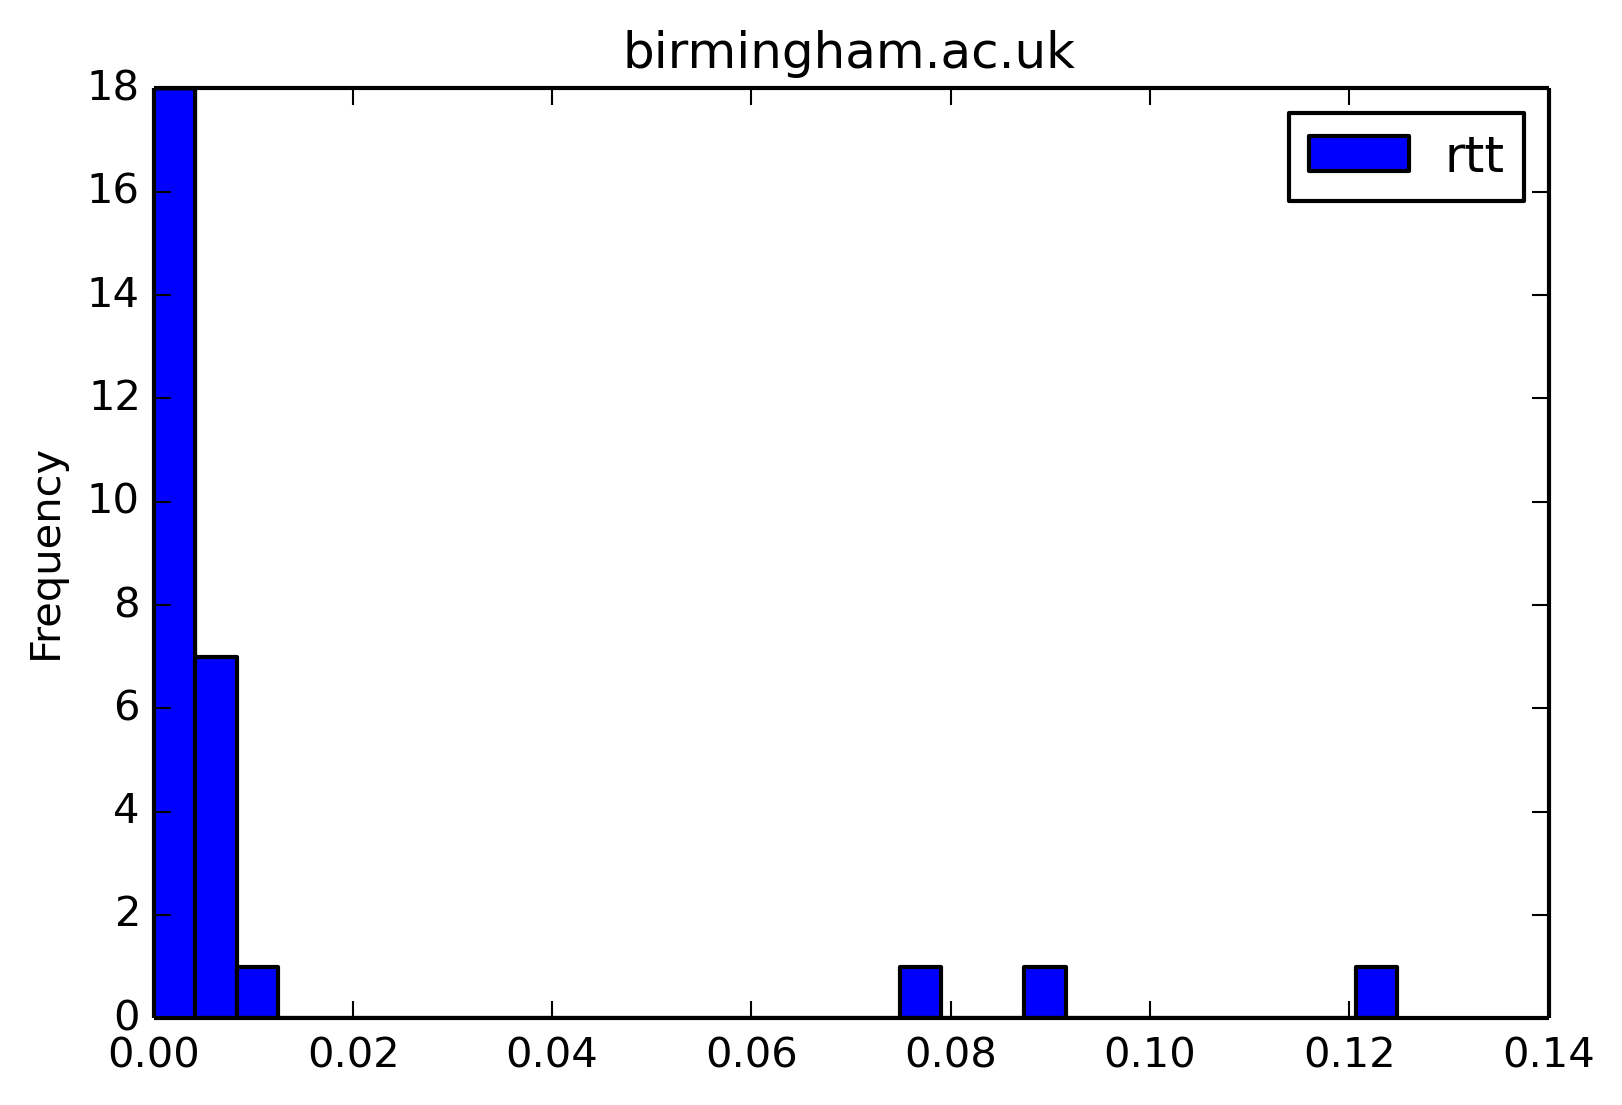
\includegraphics[width=0.45\textwidth]{histogramas_rtt/birmingham-ac-uk.png}
  \caption{RTT entre saltos}
  \label{entropia-s}
\end{figure}

\begin{figure}[H]
  \centering
    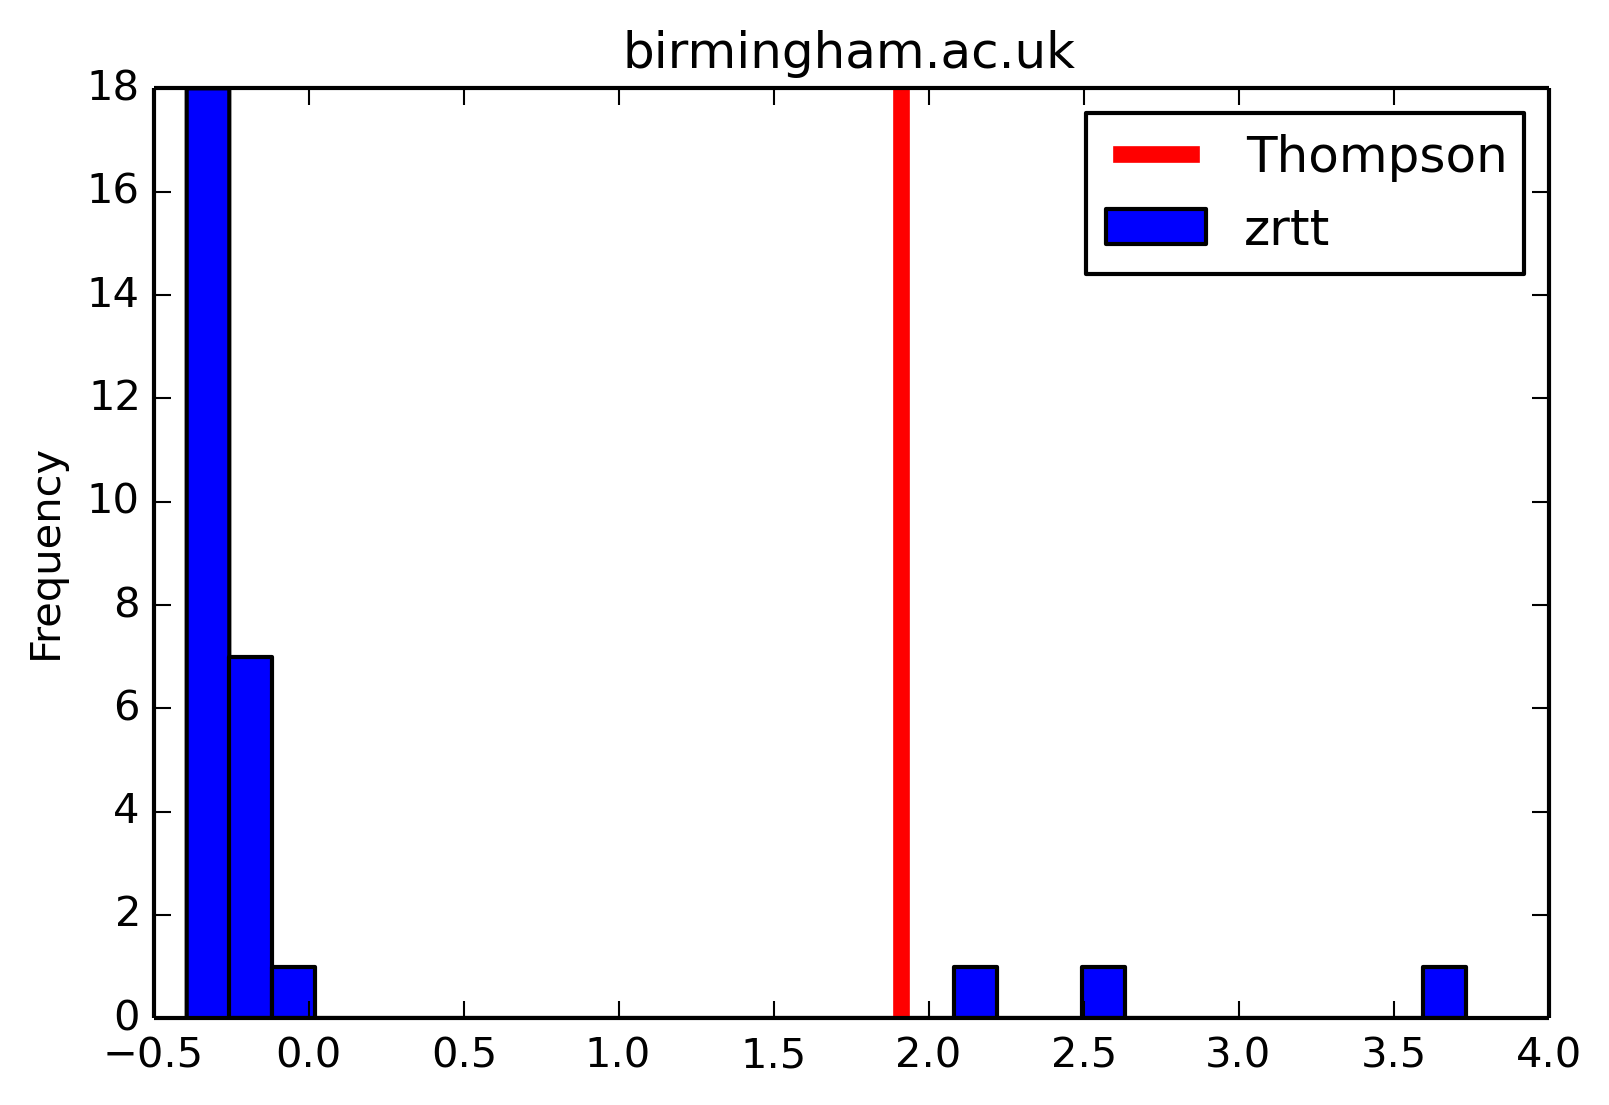
\includegraphics[width=0.45\textwidth]{histogramas_thompson/birmingham-ac-uk.png}
  \caption{RTTs Normalizados comparados con el valor Thompson}
  \label{entropia-s}
\end{figure}

\begin{figure}[H]
  \centering
    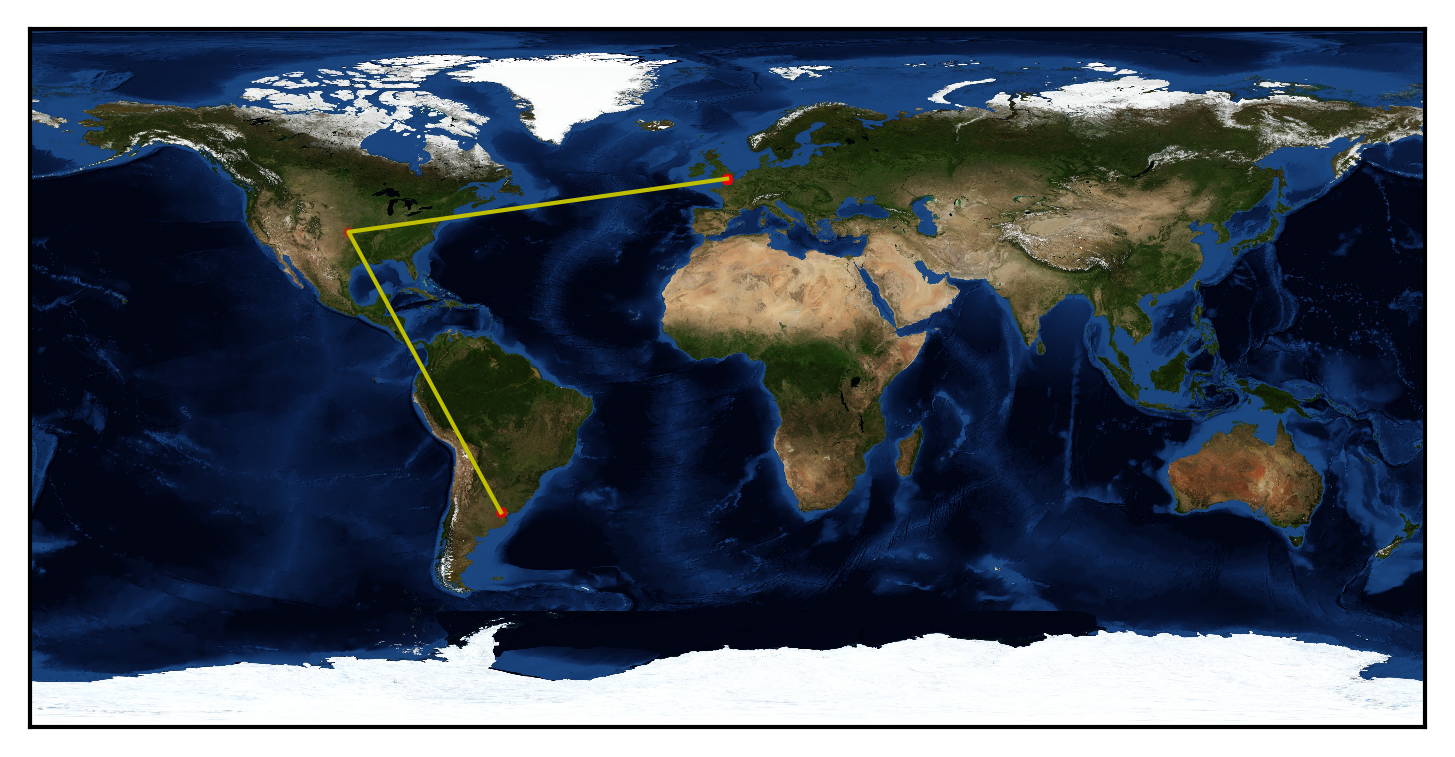
\includegraphics[width=0.45\textwidth]{grafico-rutas/birmingham-ac-uk.png}
  \caption{Gráfico de la ruta}
  \label{entropia-s}
\end{figure}